% Options for packages loaded elsewhere
\PassOptionsToPackage{unicode}{hyperref}
\PassOptionsToPackage{hyphens}{url}
%
\documentclass[
]{article}
\usepackage{amsmath,amssymb}
\usepackage{lmodern}
\usepackage{iftex}
\ifPDFTeX
  \usepackage[T1]{fontenc}
  \usepackage[utf8]{inputenc}
  \usepackage{textcomp} % provide euro and other symbols
\else % if luatex or xetex
  \usepackage{unicode-math}
  \defaultfontfeatures{Scale=MatchLowercase}
  \defaultfontfeatures[\rmfamily]{Ligatures=TeX,Scale=1}
\fi
% Use upquote if available, for straight quotes in verbatim environments
\IfFileExists{upquote.sty}{\usepackage{upquote}}{}
\IfFileExists{microtype.sty}{% use microtype if available
  \usepackage[]{microtype}
  \UseMicrotypeSet[protrusion]{basicmath} % disable protrusion for tt fonts
}{}
\makeatletter
\@ifundefined{KOMAClassName}{% if non-KOMA class
  \IfFileExists{parskip.sty}{%
    \usepackage{parskip}
  }{% else
    \setlength{\parindent}{0pt}
    \setlength{\parskip}{6pt plus 2pt minus 1pt}}
}{% if KOMA class
  \KOMAoptions{parskip=half}}
\makeatother
\usepackage{xcolor}
\usepackage[margin=1in]{geometry}
\usepackage{color}
\usepackage{fancyvrb}
\newcommand{\VerbBar}{|}
\newcommand{\VERB}{\Verb[commandchars=\\\{\}]}
\DefineVerbatimEnvironment{Highlighting}{Verbatim}{commandchars=\\\{\}}
% Add ',fontsize=\small' for more characters per line
\usepackage{framed}
\definecolor{shadecolor}{RGB}{248,248,248}
\newenvironment{Shaded}{\begin{snugshade}}{\end{snugshade}}
\newcommand{\AlertTok}[1]{\textcolor[rgb]{0.94,0.16,0.16}{#1}}
\newcommand{\AnnotationTok}[1]{\textcolor[rgb]{0.56,0.35,0.01}{\textbf{\textit{#1}}}}
\newcommand{\AttributeTok}[1]{\textcolor[rgb]{0.77,0.63,0.00}{#1}}
\newcommand{\BaseNTok}[1]{\textcolor[rgb]{0.00,0.00,0.81}{#1}}
\newcommand{\BuiltInTok}[1]{#1}
\newcommand{\CharTok}[1]{\textcolor[rgb]{0.31,0.60,0.02}{#1}}
\newcommand{\CommentTok}[1]{\textcolor[rgb]{0.56,0.35,0.01}{\textit{#1}}}
\newcommand{\CommentVarTok}[1]{\textcolor[rgb]{0.56,0.35,0.01}{\textbf{\textit{#1}}}}
\newcommand{\ConstantTok}[1]{\textcolor[rgb]{0.00,0.00,0.00}{#1}}
\newcommand{\ControlFlowTok}[1]{\textcolor[rgb]{0.13,0.29,0.53}{\textbf{#1}}}
\newcommand{\DataTypeTok}[1]{\textcolor[rgb]{0.13,0.29,0.53}{#1}}
\newcommand{\DecValTok}[1]{\textcolor[rgb]{0.00,0.00,0.81}{#1}}
\newcommand{\DocumentationTok}[1]{\textcolor[rgb]{0.56,0.35,0.01}{\textbf{\textit{#1}}}}
\newcommand{\ErrorTok}[1]{\textcolor[rgb]{0.64,0.00,0.00}{\textbf{#1}}}
\newcommand{\ExtensionTok}[1]{#1}
\newcommand{\FloatTok}[1]{\textcolor[rgb]{0.00,0.00,0.81}{#1}}
\newcommand{\FunctionTok}[1]{\textcolor[rgb]{0.00,0.00,0.00}{#1}}
\newcommand{\ImportTok}[1]{#1}
\newcommand{\InformationTok}[1]{\textcolor[rgb]{0.56,0.35,0.01}{\textbf{\textit{#1}}}}
\newcommand{\KeywordTok}[1]{\textcolor[rgb]{0.13,0.29,0.53}{\textbf{#1}}}
\newcommand{\NormalTok}[1]{#1}
\newcommand{\OperatorTok}[1]{\textcolor[rgb]{0.81,0.36,0.00}{\textbf{#1}}}
\newcommand{\OtherTok}[1]{\textcolor[rgb]{0.56,0.35,0.01}{#1}}
\newcommand{\PreprocessorTok}[1]{\textcolor[rgb]{0.56,0.35,0.01}{\textit{#1}}}
\newcommand{\RegionMarkerTok}[1]{#1}
\newcommand{\SpecialCharTok}[1]{\textcolor[rgb]{0.00,0.00,0.00}{#1}}
\newcommand{\SpecialStringTok}[1]{\textcolor[rgb]{0.31,0.60,0.02}{#1}}
\newcommand{\StringTok}[1]{\textcolor[rgb]{0.31,0.60,0.02}{#1}}
\newcommand{\VariableTok}[1]{\textcolor[rgb]{0.00,0.00,0.00}{#1}}
\newcommand{\VerbatimStringTok}[1]{\textcolor[rgb]{0.31,0.60,0.02}{#1}}
\newcommand{\WarningTok}[1]{\textcolor[rgb]{0.56,0.35,0.01}{\textbf{\textit{#1}}}}
\usepackage{longtable,booktabs,array}
\usepackage{calc} % for calculating minipage widths
% Correct order of tables after \paragraph or \subparagraph
\usepackage{etoolbox}
\makeatletter
\patchcmd\longtable{\par}{\if@noskipsec\mbox{}\fi\par}{}{}
\makeatother
% Allow footnotes in longtable head/foot
\IfFileExists{footnotehyper.sty}{\usepackage{footnotehyper}}{\usepackage{footnote}}
\makesavenoteenv{longtable}
\usepackage{graphicx}
\makeatletter
\def\maxwidth{\ifdim\Gin@nat@width>\linewidth\linewidth\else\Gin@nat@width\fi}
\def\maxheight{\ifdim\Gin@nat@height>\textheight\textheight\else\Gin@nat@height\fi}
\makeatother
% Scale images if necessary, so that they will not overflow the page
% margins by default, and it is still possible to overwrite the defaults
% using explicit options in \includegraphics[width, height, ...]{}
\setkeys{Gin}{width=\maxwidth,height=\maxheight,keepaspectratio}
% Set default figure placement to htbp
\makeatletter
\def\fps@figure{htbp}
\makeatother
\setlength{\emergencystretch}{3em} % prevent overfull lines
\providecommand{\tightlist}{%
  \setlength{\itemsep}{0pt}\setlength{\parskip}{0pt}}
\setcounter{secnumdepth}{-\maxdimen} % remove section numbering
\ifLuaTeX
  \usepackage{selnolig}  % disable illegal ligatures
\fi
\IfFileExists{bookmark.sty}{\usepackage{bookmark}}{\usepackage{hyperref}}
\IfFileExists{xurl.sty}{\usepackage{xurl}}{} % add URL line breaks if available
\urlstyle{same} % disable monospaced font for URLs
\hypersetup{
  hidelinks,
  pdfcreator={LaTeX via pandoc}}

\title{\textbf{\emph{``S7 Dependencia de los celulares en estudiantes
universitarios''}}}
\author{}
\date{\vspace{-2.5em}}

\begin{document}
\maketitle

\begin{enumerate}
\def\labelenumi{\arabic{enumi}.}
\item
\end{enumerate}

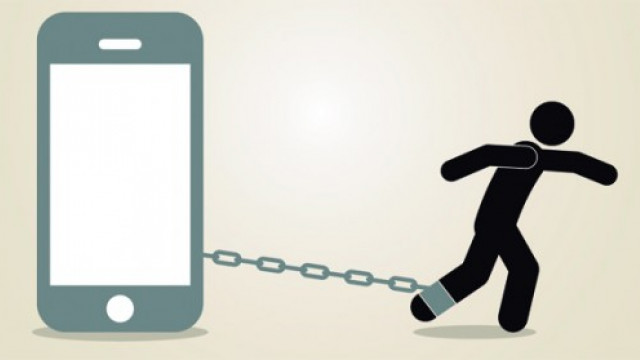
\includegraphics{captura2.jpg}

\textbf{\emph{Integrantes:}}

\begin{longtable}[]{@{}lc@{}}
\toprule()
\textbf{Nombres y apellidos} & \textbf{Código} \\
\midrule()
\endhead
Cabello Guerrero, Fabrizzio Raphael \textbf{(líder)} & 202120116 \\
Casma morales, Hosmer Gilberto & 20202026 \\
Dávila Loa, Ana María Isabel & 202210606 \\
Espinoza Portillo, Gean Franco & 202120635 \\
Salvador Ñiques, Alexander Fernand & 201920139 \\
\bottomrule()
\end{longtable}

\textbf{\emph{Profesora: Cornejo Villena, Hugo}}

\textbf{Teo.13 - Lab.13.01}

\hypertarget{tuxedtulo-del-proyecto}{%
\subsection{Título del proyecto}\label{tuxedtulo-del-proyecto}}

\textbf{Dependencia de los celulares en estudiantes universitarios}

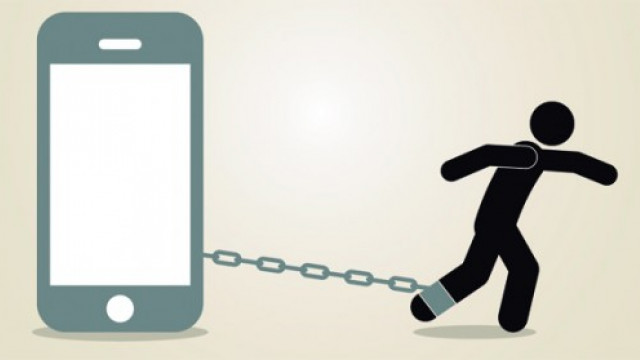
\includegraphics{captura2.jpg}

\hypertarget{i.-introducciuxf3n}{%
\subsection{I. Introducción}\label{i.-introducciuxf3n}}

En los últimos años, la tecnología está formando parte de nuestra vida
cotidiana. Para ser más precisos, los celulares están siendo los
protagonistas Debido a que cada vez las personas tienen la necesidad de
adquirir un equipo para estar comunicados con los demás. Pero cuando la
relación entre persona y celular se vuelve dependiente es donde afloran
los problemas.Bajo ese contexto son los jóvenes quienes actualmente
están más pendientes del celular debido a los estudios, trabajo, momento
de ocio etc. Es por ello que estudiamos la problemática de la
dependencia del celular para conocer con que incidencia influye en la
persona.

\hypertarget{planificaciuxf3n}{%
\subsubsection{1.1 Planificación}\label{planificaciuxf3n}}

\hypertarget{ii.-datos}{%
\subsection{II. Datos}\label{ii.-datos}}

\hypertarget{recolecciuxf3n-de-datos}{%
\subsubsection{2.1 Recolección de
datos:}\label{recolecciuxf3n-de-datos}}

\hypertarget{proceso-de-recolecciuxf3n-de-datos}{%
\subsubsection{\texorpdfstring{\textbf{Proceso de recolección de
datos}}{Proceso de recolección de datos}}\label{proceso-de-recolecciuxf3n-de-datos}}

La recolección de datos para esta investigación fue gracias a las
encuestas repartidas a los diferentes estudiantes de la universidad
\textbf{UTEC}. Nos inclinamos al uso de las encuestas ya que es una
buena herramienta que nos ayudaría a conocer ciertas informaciones
relevantes que requerimos para nuestra investigación. En esta ocasión no
hubo restricción para nuestra muestra estadística ya que todos los
alumnos de \textbf{UTEC} pueden formar parte de ella. Las estrategias
que se utilizaron para la recolección de los datos fue las dinámicas de
los integrantes para que los estudiados accedieran a llenar las
encuestas y pedir amablemente los datos que también son brindados por
los celulares de cada muestra, todo esto a diferentes horas en los
transcurrir de los días. De esta forma pudimos concluir con una buena
recolección de datos además de un excelente trabajo en equipo.

\hypertarget{poblaciuxf3n-muestra-y-muestreo}{%
\subsubsection{\texorpdfstring{\textbf{Población, muestra y
muestreo}}{Población, muestra y muestreo}}\label{poblaciuxf3n-muestra-y-muestreo}}

\begin{itemize}
\item
  \textbf{Población de estudio}\\
  La población de estudio del proyecto es infinita, ya que no se conoce
  el número exacto de la población a estudiar. Está representada por
  todos los alumnos de UTEC para el tema a tratar en el proyecto que es
  la dependencia del uso de celulares en relación con los estudiantes de
  la UTEC.
\item
  \textbf{Unidad muestral}\\
  La unidad muestral es un alumno de UTEC. De este estamos interesados
  en analizar variables como el tiempo que le dedica al uso del celular,
  el tiempo de carga de este y el tiempo que dedica a las redes sociales
  entre otros.
\item
  \textbf{Muestra}\\
  El tamaño de la muestra a analizar es de 63 alumnos. El nivel de
  confianza (NC) elegido es del 90\%. El error estimado (e) es del 10\%.
  El porcentaje de aceptación de proporción esperada de la muestra es de
  35\%.
\item
  \textbf{Muestreo}\\
  La muestra es representativa porque tiene un nivel de confianza y un
  margen de error. Además, para seleccionar a los elementos de la
  muestra se utilizó la modalidad de muestreo con selección aleatoria
  simple para garantizar la equisprobabilidad de elección de cualquier
  elemento.
\end{itemize}

\hypertarget{variables}{%
\subsubsection{\texorpdfstring{\textbf{Variables}}{Variables}}\label{variables}}

\begin{longtable}[]{@{}
  >{\raggedright\arraybackslash}p{(\columnwidth - 4\tabcolsep) * \real{0.3333}}
  >{\raggedright\arraybackslash}p{(\columnwidth - 4\tabcolsep) * \real{0.3333}}
  >{\raggedright\arraybackslash}p{(\columnwidth - 4\tabcolsep) * \real{0.3333}}@{}}
\toprule()
\begin{minipage}[b]{\linewidth}\raggedright
Variable de estudio
\end{minipage} & \begin{minipage}[b]{\linewidth}\raggedright
Tipo de variables
\end{minipage} & \begin{minipage}[b]{\linewidth}\raggedright
Restricción
\end{minipage} \\
\midrule()
\endhead
Edad & Tipo numérica discreta y es un entero positivo & 16 \textless{}
Edad \textless{} 30 \\
Sexo & Tipo categórica nominal & Masculino o Femenino \\
Carrera & Tipo categórica de nominal & Carreras en UTEC \\
Dispositivo con Frecuencia & Tipo categórica de nominal & Celular,
tablet, PC, laptop, relojes inteligentes \\
promedio del uso del celular al día & Tipo numeria discreta y números
enteros positivos & 240 \textless{} Minutos \textless{} 500 \\
promedio de la bateria del celular & Tipo numeria discreta y números
enteros positivos & 900 \textless{} Minutos \textless{} 1080 \\
Edad cuando tuviste tu primer celular & Tipo numérica discretas y
números enteros positivos & 5 \textless{} Edad \textless{} 30 \\
Tiempo de carga de la batería & Tipo numérica discretas y números
enteros positivos & 100 \textless{} Minutos \textgreater{} 360 \\
Tiempo que le dedicas a las redes sociales & Tipo numérica discreta y
números enteros positivos & 20 \textless{} Minutos \textgreater{} 240 \\
Tiempo que dejas de usar el celular & Tipo numérica discretas y números
enteros positivos & 180 \textless{} Minutos \textgreater{} 600 \\
Nivel de angustia sin celular & Tipo Categoria ordinal y números enteros
positivos del 1 al 5 & Escala del 1 al 5 \\
Nivel de angustia con bateria baja del celular & Tipo Categoria ordinal
y números enteros positivos del 1 al 5 & Escala del 1 al 5 \\
nivel de importancia del celular y los estudios & Tipo Categoria ordinal
y números enteros positivos del 1 al 5 & Escala del 1 al 5 \\
nivel de frecuencia del uso de videojuegos & Tipo Categoria ordinal y
números enteros positivos del 1 al 5 & Escala del 1 al 5 \\
Lugar donde usas mayormente tu celular & Tipo categórica nominal & Casa,
cubículo, salón de clases sala de estudio, baños, ambiente del piso 6,
laboratorios, pasillos de UTEC, en los medios de transporte \\
Tiempo de espera para usar el celular despues de dejarlo cargando & Tipo
numérica discretas y números enteros positivos & 1 \textless{} Minutos
\textgreater{} 60 \\
Tiempo del uso del celular despues de dejarlo cargando segun el celular
& Tipo numérica discretas y números enteros positivos & 20 \textless{}
Minutos \textgreater{} 240 \\
Tiempo de duracion del celular desde la ultima carga segun el celular &
Tipo numérica discretas y números enteros positivos & 180 \textless{}
Minutos \textgreater{} 480 \\
Tiempo de no uso del celular segun el celular & Tipo numérica discretas
y números enteros positivos & 120 \textless{} Minutos \textgreater{}
300 \\
\bottomrule()
\end{longtable}

\hypertarget{limpieza-de-base-de-datos}{%
\subsubsection{2.4 Limpieza de base de
datos:}\label{limpieza-de-base-de-datos}}

\textbf{- Librerías a usar para la lectura de la data}

\begin{Shaded}
\begin{Highlighting}[]
\FunctionTok{library}\NormalTok{(readr)}
\end{Highlighting}
\end{Shaded}

\begin{verbatim}
## Warning: package 'readr' was built under R version 4.2.2
\end{verbatim}

\begin{Shaded}
\begin{Highlighting}[]
\FunctionTok{library}\NormalTok{(dplyr)}
\end{Highlighting}
\end{Shaded}

\begin{verbatim}
## 
## Attaching package: 'dplyr'
\end{verbatim}

\begin{verbatim}
## The following objects are masked from 'package:stats':
## 
##     filter, lag
\end{verbatim}

\begin{verbatim}
## The following objects are masked from 'package:base':
## 
##     intersect, setdiff, setequal, union
\end{verbatim}

\begin{Shaded}
\begin{Highlighting}[]
\FunctionTok{library}\NormalTok{(modeest)}
\end{Highlighting}
\end{Shaded}

\begin{verbatim}
## Warning: package 'modeest' was built under R version 4.2.2
\end{verbatim}

\begin{Shaded}
\begin{Highlighting}[]
\FunctionTok{library}\NormalTok{(foreign)}
\FunctionTok{library}\NormalTok{(fitdistrplus)}
\end{Highlighting}
\end{Shaded}

\begin{verbatim}
## Warning: package 'fitdistrplus' was built under R version 4.2.2
\end{verbatim}

\begin{verbatim}
## Loading required package: MASS
\end{verbatim}

\begin{verbatim}
## Warning: package 'MASS' was built under R version 4.2.2
\end{verbatim}

\begin{verbatim}
## 
## Attaching package: 'MASS'
\end{verbatim}

\begin{verbatim}
## The following object is masked from 'package:dplyr':
## 
##     select
\end{verbatim}

\begin{verbatim}
## Loading required package: survival
\end{verbatim}

\begin{Shaded}
\begin{Highlighting}[]
\FunctionTok{library}\NormalTok{(ggplot2)}
\end{Highlighting}
\end{Shaded}

\begin{verbatim}
## Warning: package 'ggplot2' was built under R version 4.2.2
\end{verbatim}

\textbf{- Lectura de la data}

\begin{Shaded}
\begin{Highlighting}[]
\NormalTok{DF }\OtherTok{\textless{}{-}} \FunctionTok{read\_csv}\NormalTok{(}\StringTok{"Datos.csv"}\NormalTok{)}
\end{Highlighting}
\end{Shaded}

\begin{verbatim}
## New names:
## Rows: 202 Columns: 21
## -- Column specification
## -------------------------------------------------------- Delimiter: "," chr
## (6): Marca temporal, Sexo, Carrera, ¿Qué tipo de dispositivo usas con m... dbl
## (15): Edad (años), ¿Cuánto tiempo, en promedio, usas tu celular al día? ...
## i Use `spec()` to retrieve the full column specification for this data. i
## Specify the column types or set `show_col_types = FALSE` to quiet this message.
## * `` -> `...21`
\end{verbatim}

\begin{Shaded}
\begin{Highlighting}[]
\FunctionTok{spec}\NormalTok{(DF)}
\end{Highlighting}
\end{Shaded}

\begin{verbatim}
## cols(
##   `Marca temporal` = col_character(),
##   `Edad (años)` = col_double(),
##   Sexo = col_character(),
##   Carrera = col_character(),
##   `¿Qué tipo de dispositivo usas con mayor  frecuencia?` = col_character(),
##   `¿Cuánto tiempo, en promedio, usas tu celular al día? En minutos (Recordar: 1 hora = 60 minutos)` = col_double(),
##   `¿Cuánto dura, en promedio, la batería de tu celular?  En minutos (Recordar: 1 hora = 60 minutos)` = col_double(),
##   `¿A qué edad usaste tu primer celular? En años (Ejemplo: 18)` = col_double(),
##   `Después de que se descarga tu celular, ¿por cuánto tiempo, en promedio, lo dejas cargando? En minutos (Recordar: 1 hora = 60 minutos)` = col_double(),
##   `¿Cuánto tiempo, en promedio, le dedicas a las redes sociales al día? En minutos  (Recordar: 1 hora = 60 minutos)` = col_double(),
##   `¿Por cuánto tiempo, en promedio, dejas de usar tu celular al día? En minutos.` = col_double(),
##   `Nivel de angustia sin celular: 1 nada angustiado y 5 muy angustiado.` = col_double(),
##   `¿Qué tan angustiado te sientes al ver tu celular con baja bateria?  1 Nada angustiado y 5 Muy angustiado.` = col_double(),
##   `¿Qué nivel de importancia tiene usar tu celular para tus estudios?  1 Nada importante y 5 Muy importante.` = col_double(),
##   `¿Con qué frecuencia juegas videojuegos? 1 Nada frecuente y 5 Muy frecuente.` = col_double(),
##   `¿En qué lugar usas mayormente tu celular?` = col_character(),
##   `¿Cuántos minutos esperas para volver a usar tu celular luego de dejarlo cargando? (en minutos)` = col_double(),
##   `¿Cuánto tiempo usaste tu celular desde la última carga, segun tu celular? (en minutos)` = col_double(),
##   `¿Cuánto tiempo de duración tiene tu batería desde tu ultima carga, segun tu celular?  En minutos (Recordar: 1 hora = 60 minutos)` = col_double(),
##   `¿Cuánto tiempo no usas tu celular en el día, segun tu celular? (en minutos)` = col_double(),
##   ...21 = col_character()
## )
\end{verbatim}

\textbf{- Renombramiento de las variables}

\begin{Shaded}
\begin{Highlighting}[]
\NormalTok{DF }\SpecialCharTok{\%\textgreater{}\%}\FunctionTok{rename}\NormalTok{(}\AttributeTok{Edad =} \StringTok{\textasciigrave{}}\AttributeTok{Edad (años)}\StringTok{\textasciigrave{}}\NormalTok{,}
\AttributeTok{Sexo =}\NormalTok{ Sexo, }

\AttributeTok{Carrera=}\NormalTok{ Carrera,}
             
\AttributeTok{Dispositivo =} \StringTok{\textasciigrave{}}\AttributeTok{¿Qué tipo de dispositivo usas con mayor  frecuencia?}\StringTok{\textasciigrave{}}\NormalTok{,}

\AttributeTok{Uso\_del\_celular\_dia =} \StringTok{\textasciigrave{}}\AttributeTok{¿Cuánto tiempo, en promedio, usas tu celular al día? En minutos (Recordar: 1 hora = 60 minutos)}\StringTok{\textasciigrave{}}\NormalTok{,}

\AttributeTok{Duracion\_de\_bateria =} \StringTok{\textasciigrave{}}\AttributeTok{¿Cuánto dura, en promedio, la batería de tu celular?  En minutos (Recordar: 1 hora = 60 minutos)}\StringTok{\textasciigrave{}}\NormalTok{,}
             
\AttributeTok{Edad\_del\_primero\_celular =} \StringTok{\textasciigrave{}}\AttributeTok{¿A qué edad usaste tu primer celular? En años (Ejemplo: 18)}\StringTok{\textasciigrave{}}\NormalTok{, }

\AttributeTok{Tiempo\_de\_carga =} \StringTok{\textasciigrave{}}\AttributeTok{Después de que se descarga tu celular, ¿por cuánto tiempo, en promedio, lo dejas cargando? En minutos (Recordar: 1 hora = 60 minutos)}\StringTok{\textasciigrave{}}\NormalTok{,}

\AttributeTok{Redes\_sociales =} \StringTok{\textasciigrave{}}\AttributeTok{¿Cuánto tiempo, en promedio, le dedicas a las redes sociales al día? En minutos  (Recordar: 1 hora = 60 minutos)}\StringTok{\textasciigrave{}}\NormalTok{,}

\AttributeTok{Dejar\_el\_celular =} \StringTok{\textasciigrave{}}\AttributeTok{¿Por cuánto tiempo, en promedio, dejas de usar tu celular al día? En minutos.}\StringTok{\textasciigrave{}}\NormalTok{,}

\AttributeTok{Angustia\_sin\_celular=} \StringTok{\textasciigrave{}}\AttributeTok{Nivel de angustia sin celular: 1 nada angustiado y 5 muy angustiado.}\StringTok{\textasciigrave{}}\NormalTok{, }

\AttributeTok{Angustia\_bateria\_baja=} \StringTok{\textasciigrave{}}\AttributeTok{¿Qué tan angustiado te sientes al ver tu celular con baja bateria?  1 Nada angustiado y 5 Muy angustiado.}\StringTok{\textasciigrave{}}\NormalTok{, }

\AttributeTok{Importancia\_de\_usar\_celuar =} \StringTok{\textasciigrave{}}\AttributeTok{¿Qué nivel de importancia tiene usar tu celular para tus estudios?  1 Nada importante y 5 Muy importante.}\StringTok{\textasciigrave{}}\NormalTok{,}

\AttributeTok{Frecuencia\_de\_videojuegos=} \StringTok{\textasciigrave{}}\AttributeTok{¿Con qué frecuencia juegas videojuegos? 1 Nada frecuente y 5 Muy frecuente.}\StringTok{\textasciigrave{}}\NormalTok{, }

\AttributeTok{lugar\_uso =} \StringTok{\textasciigrave{}}\AttributeTok{¿En qué lugar usas mayormente tu celular?}\StringTok{\textasciigrave{}}\NormalTok{,}

\AttributeTok{Tiempo\_de\_espera=}\StringTok{\textasciigrave{}}\AttributeTok{¿Cuántos minutos esperas para volver a usar tu celular luego de dejarlo cargando? (en minutos)}\StringTok{\textasciigrave{}}\NormalTok{,}

\AttributeTok{Uso\_del\_celular\_Utimacarga=}\StringTok{\textasciigrave{}}\AttributeTok{¿Cuánto tiempo usaste tu celular desde la última carga, segun tu celular? (en minutos)}\StringTok{\textasciigrave{}}\NormalTok{,}

\AttributeTok{Duracion\_bateria\_segun\_cel=}\StringTok{\textasciigrave{}}\AttributeTok{¿Cuánto tiempo de duración tiene tu batería desde tu ultima carga, segun tu celular?  En minutos (Recordar: 1 hora = 60 minutos)}\StringTok{\textasciigrave{}}\NormalTok{,}

\AttributeTok{Tiempo\_sin\_celular=}\StringTok{\textasciigrave{}}\AttributeTok{¿Cuánto tiempo no usas tu celular en el día, segun tu celular? (en minutos)}\StringTok{\textasciigrave{}}\NormalTok{)}\OtherTok{{-}\textgreater{}}\NormalTok{ DFN}
\end{Highlighting}
\end{Shaded}

\textbf{- Limpieza de datos}

\begin{Shaded}
\begin{Highlighting}[]
\FunctionTok{summary}\NormalTok{(DFN)}
\end{Highlighting}
\end{Shaded}

\begin{verbatim}
##  Marca temporal          Edad           Sexo             Carrera         
##  Length:202         Min.   :16.00   Length:202         Length:202        
##  Class :character   1st Qu.:19.00   Class :character   Class :character  
##  Mode  :character   Median :20.00   Mode  :character   Mode  :character  
##                     Mean   :20.73                                        
##                     3rd Qu.:22.00                                        
##                     Max.   :34.00                                        
##  Dispositivo        Uso_del_celular_dia Duracion_de_bateria
##  Length:202         Min.   :120.0       Min.   : 100.0     
##  Class :character   1st Qu.:250.0       1st Qu.: 930.0     
##  Mode  :character   Median :330.0       Median : 962.0     
##                     Mean   :344.6       Mean   : 935.6     
##                     3rd Qu.:420.0       3rd Qu.:1020.0     
##                     Max.   :720.0       Max.   :1600.0     
##  Edad_del_primero_celular Tiempo_de_carga Redes_sociales   Dejar_el_celular
##  Min.   : 5.00            Min.   : 20.0   Min.   : 20.00   Min.   :  30.0  
##  1st Qu.:11.00            1st Qu.:125.0   1st Qu.: 51.25   1st Qu.: 187.0  
##  Median :13.00            Median :180.0   Median :100.00   Median : 330.0  
##  Mean   :12.93            Mean   :198.5   Mean   :125.88   Mean   : 331.9  
##  3rd Qu.:15.00            3rd Qu.:247.5   3rd Qu.:190.00   3rd Qu.: 497.5  
##  Max.   :25.00            Max.   :480.0   Max.   :500.00   Max.   :1200.0  
##  Angustia_sin_celular Angustia_bateria_baja Importancia_de_usar_celuar
##  Min.   :1.00         Min.   :1.000         Min.   :1.00              
##  1st Qu.:3.00         1st Qu.:2.000         1st Qu.:3.00              
##  Median :4.00         Median :4.000         Median :4.00              
##  Mean   :3.46         Mean   :3.312         Mean   :3.51              
##  3rd Qu.:4.00         3rd Qu.:4.000         3rd Qu.:4.00              
##  Max.   :5.00         Max.   :5.000         Max.   :5.00              
##  Frecuencia_de_videojuegos  lugar_uso         Tiempo_de_espera
##  Min.   :1.000             Length:202         Min.   :  1.00  
##  1st Qu.:2.000             Class :character   1st Qu.: 30.00  
##  Median :3.000             Mode  :character   Median : 40.00  
##  Mean   :3.015                                Mean   : 45.31  
##  3rd Qu.:4.000                                3rd Qu.: 50.00  
##  Max.   :5.000                                Max.   :300.00  
##  Uso_del_celular_Utimacarga Duracion_bateria_segun_cel Tiempo_sin_celular
##  Min.   : 15.0              Min.   :  50.0             Min.   : 30.0     
##  1st Qu.:104.8              1st Qu.: 203.0             1st Qu.:150.0     
##  Median :150.0              Median : 262.0             Median :195.5     
##  Mean   :153.1              Mean   : 287.6             Mean   :215.9     
##  3rd Qu.:200.0              3rd Qu.: 340.8             3rd Qu.:256.8     
##  Max.   :547.0              Max.   :2274.0             Max.   :912.0     
##     ...21          
##  Length:202        
##  Class :character  
##  Mode  :character  
##                    
##                    
## 
\end{verbatim}

\textbf{Verificacion}

\begin{Shaded}
\begin{Highlighting}[]
\FunctionTok{summary}\NormalTok{(DFN)}
\end{Highlighting}
\end{Shaded}

\begin{verbatim}
##  Marca temporal          Edad           Sexo             Carrera         
##  Length:202         Min.   :16.00   Length:202         Length:202        
##  Class :character   1st Qu.:19.00   Class :character   Class :character  
##  Mode  :character   Median :20.00   Mode  :character   Mode  :character  
##                     Mean   :20.73                                        
##                     3rd Qu.:22.00                                        
##                     Max.   :34.00                                        
##  Dispositivo        Uso_del_celular_dia Duracion_de_bateria
##  Length:202         Min.   :120.0       Min.   : 100.0     
##  Class :character   1st Qu.:250.0       1st Qu.: 930.0     
##  Mode  :character   Median :330.0       Median : 962.0     
##                     Mean   :344.6       Mean   : 935.6     
##                     3rd Qu.:420.0       3rd Qu.:1020.0     
##                     Max.   :720.0       Max.   :1600.0     
##  Edad_del_primero_celular Tiempo_de_carga Redes_sociales   Dejar_el_celular
##  Min.   : 5.00            Min.   : 20.0   Min.   : 20.00   Min.   :  30.0  
##  1st Qu.:11.00            1st Qu.:125.0   1st Qu.: 51.25   1st Qu.: 187.0  
##  Median :13.00            Median :180.0   Median :100.00   Median : 330.0  
##  Mean   :12.93            Mean   :198.5   Mean   :125.88   Mean   : 331.9  
##  3rd Qu.:15.00            3rd Qu.:247.5   3rd Qu.:190.00   3rd Qu.: 497.5  
##  Max.   :25.00            Max.   :480.0   Max.   :500.00   Max.   :1200.0  
##  Angustia_sin_celular Angustia_bateria_baja Importancia_de_usar_celuar
##  Min.   :1.00         Min.   :1.000         Min.   :1.00              
##  1st Qu.:3.00         1st Qu.:2.000         1st Qu.:3.00              
##  Median :4.00         Median :4.000         Median :4.00              
##  Mean   :3.46         Mean   :3.312         Mean   :3.51              
##  3rd Qu.:4.00         3rd Qu.:4.000         3rd Qu.:4.00              
##  Max.   :5.00         Max.   :5.000         Max.   :5.00              
##  Frecuencia_de_videojuegos  lugar_uso         Tiempo_de_espera
##  Min.   :1.000             Length:202         Min.   :  1.00  
##  1st Qu.:2.000             Class :character   1st Qu.: 30.00  
##  Median :3.000             Mode  :character   Median : 40.00  
##  Mean   :3.015                                Mean   : 45.31  
##  3rd Qu.:4.000                                3rd Qu.: 50.00  
##  Max.   :5.000                                Max.   :300.00  
##  Uso_del_celular_Utimacarga Duracion_bateria_segun_cel Tiempo_sin_celular
##  Min.   : 15.0              Min.   :  50.0             Min.   : 30.0     
##  1st Qu.:104.8              1st Qu.: 203.0             1st Qu.:150.0     
##  Median :150.0              Median : 262.0             Median :195.5     
##  Mean   :153.1              Mean   : 287.6             Mean   :215.9     
##  3rd Qu.:200.0              3rd Qu.: 340.8             3rd Qu.:256.8     
##  Max.   :547.0              Max.   :2274.0             Max.   :912.0     
##     ...21          
##  Length:202        
##  Class :character  
##  Mode  :character  
##                    
##                    
## 
\end{verbatim}

\hypertarget{descriptor-grafico}{%
\subsection{- Descriptor grafico}\label{descriptor-grafico}}

\textbf{Variable edad}

\begin{Shaded}
\begin{Highlighting}[]
\NormalTok{Tabla }\OtherTok{\textless{}{-}}\NormalTok{ DFN}\SpecialCharTok{\%\textgreater{}\%} \FunctionTok{group\_by}\NormalTok{(Sexo) }\SpecialCharTok{\%\textgreater{}\%} \FunctionTok{summarise}\NormalTok{(}\AttributeTok{Total=}\FunctionTok{n}\NormalTok{())   }
    
\FunctionTok{ggplot}\NormalTok{(Tabla, }\FunctionTok{aes}\NormalTok{(}\AttributeTok{x =}\NormalTok{ Sexo, }\AttributeTok{y=}\NormalTok{Total,}\AttributeTok{fill=}\NormalTok{Sexo) ) }\SpecialCharTok{+}    
  \FunctionTok{geom\_bar}\NormalTok{(}\AttributeTok{width =} \FloatTok{0.9}\NormalTok{, }\AttributeTok{stat=}\StringTok{"identity"}\NormalTok{,              }
           \AttributeTok{position =} \FunctionTok{position\_dodge}\NormalTok{()                 )}\SpecialCharTok{+}  
  
  \FunctionTok{ylim}\NormalTok{(}\FunctionTok{c}\NormalTok{(}\DecValTok{0}\NormalTok{,}\DecValTok{200}\NormalTok{))}\SpecialCharTok{+}
  \FunctionTok{labs}\NormalTok{(}\AttributeTok{x=}\StringTok{"Sexo de los encuestados"}\NormalTok{, }\AttributeTok{y=} \StringTok{"Frecuencia"}\NormalTok{) }\SpecialCharTok{+}   
  \FunctionTok{labs}\NormalTok{(}\AttributeTok{fill =} \StringTok{""}\NormalTok{)}\SpecialCharTok{+}                                         
  
  \FunctionTok{geom\_text}\NormalTok{(}\FunctionTok{aes}\NormalTok{(}\AttributeTok{label=}\NormalTok{Total), }\AttributeTok{vjust=}\FloatTok{1.6}\NormalTok{, }\AttributeTok{color=}\StringTok{"black"}\NormalTok{,    }
              \AttributeTok{position =} \FunctionTok{position\_dodge}\NormalTok{(}\FloatTok{0.9}\NormalTok{),  }\AttributeTok{size=}\FloatTok{4.0}
\NormalTok{            ) }\SpecialCharTok{+}                                            
  
  \FunctionTok{theme\_bw}\NormalTok{(}\AttributeTok{base\_size =} \DecValTok{15}\NormalTok{)}
\end{Highlighting}
\end{Shaded}

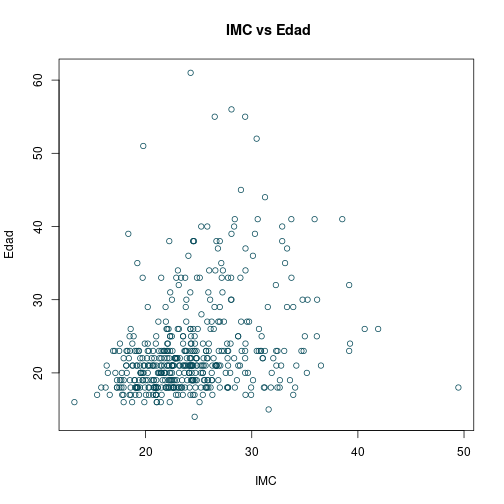
\includegraphics{S7_Infomre_E2_files/figure-latex/unnamed-chunk-7-1.pdf}

\textbf{Dispositivos}

``Falta agregar titulo''

\begin{Shaded}
\begin{Highlighting}[]
\NormalTok{Tabla }\OtherTok{\textless{}{-}}\NormalTok{ DFN}\SpecialCharTok{\%\textgreater{}\%} \FunctionTok{group\_by}\NormalTok{(Carrera) }\SpecialCharTok{\%\textgreater{}\%} \FunctionTok{summarise}\NormalTok{(}\AttributeTok{Total=}\FunctionTok{n}\NormalTok{())   }
    
\FunctionTok{ggplot}\NormalTok{(Tabla, }\FunctionTok{aes}\NormalTok{(}\AttributeTok{x =} \StringTok{"Carreras"}\NormalTok{, }\AttributeTok{y=}\NormalTok{Total,}\AttributeTok{fill=}\NormalTok{Carrera) ) }\SpecialCharTok{+}    
  \FunctionTok{geom\_bar}\NormalTok{(}\AttributeTok{width =} \FloatTok{1.5}\NormalTok{, }\AttributeTok{stat=}\StringTok{"identity"}\NormalTok{,              }
           \AttributeTok{position =} \FunctionTok{position\_dodge}\NormalTok{()                 )}\SpecialCharTok{+}  
  
  \FunctionTok{ylim}\NormalTok{(}\FunctionTok{c}\NormalTok{(}\DecValTok{0}\NormalTok{,}\DecValTok{30}\NormalTok{))}\SpecialCharTok{+}
  \FunctionTok{labs}\NormalTok{(}\AttributeTok{x=}\StringTok{"Carreras de los encuestados"}\NormalTok{, }\AttributeTok{y=} \StringTok{"Frecuencia"}\NormalTok{) }\SpecialCharTok{+}   
  \FunctionTok{labs}\NormalTok{(}\AttributeTok{fill =} \StringTok{""}\NormalTok{)}\SpecialCharTok{+}                                         
  
  \FunctionTok{geom\_text}\NormalTok{(}\FunctionTok{aes}\NormalTok{(}\AttributeTok{label=}\NormalTok{Total), }\AttributeTok{vjust=}\FloatTok{1.6}\NormalTok{, }\AttributeTok{color=}\StringTok{"black"}\NormalTok{,    }
              \AttributeTok{position =} \FunctionTok{position\_dodge}\NormalTok{(}\FloatTok{1.5}\NormalTok{),  }\AttributeTok{size=}\FloatTok{4.0}
\NormalTok{            ) }\SpecialCharTok{+}                                            
  
  \FunctionTok{theme\_bw}\NormalTok{(}\AttributeTok{base\_size =} \DecValTok{10}\NormalTok{)}
\end{Highlighting}
\end{Shaded}

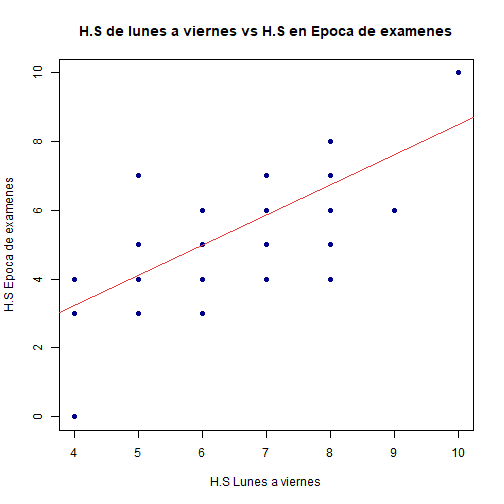
\includegraphics{S7_Infomre_E2_files/figure-latex/unnamed-chunk-8-1.pdf}

\textbf{Lugar de uso}

``Falta agregar titulo''

\begin{Shaded}
\begin{Highlighting}[]
\NormalTok{Tabla }\OtherTok{\textless{}{-}}\NormalTok{ DFN}\SpecialCharTok{\%\textgreater{}\%} \FunctionTok{group\_by}\NormalTok{(lugar\_uso) }\SpecialCharTok{\%\textgreater{}\%} \FunctionTok{summarise}\NormalTok{(}\AttributeTok{Total=}\FunctionTok{n}\NormalTok{())   }
    
\FunctionTok{ggplot}\NormalTok{(Tabla, }\FunctionTok{aes}\NormalTok{(}\AttributeTok{x =} \StringTok{"Lugar de uso"}\NormalTok{, }\AttributeTok{y=}\NormalTok{Total,}\AttributeTok{fill=}\NormalTok{lugar\_uso) ) }\SpecialCharTok{+}    
  \FunctionTok{geom\_bar}\NormalTok{(}\AttributeTok{width =} \FloatTok{0.9}\NormalTok{, }\AttributeTok{stat=}\StringTok{"identity"}\NormalTok{,              }
           \AttributeTok{position =} \FunctionTok{position\_dodge}\NormalTok{()                 )}\SpecialCharTok{+}  
  
  \FunctionTok{ylim}\NormalTok{(}\FunctionTok{c}\NormalTok{(}\DecValTok{0}\NormalTok{,}\DecValTok{40}\NormalTok{))}\SpecialCharTok{+}
  \FunctionTok{labs}\NormalTok{(}\AttributeTok{x=}\StringTok{"Dispositivos de los encuestados"}\NormalTok{, }\AttributeTok{y=} \StringTok{"Frecuencia"}\NormalTok{) }\SpecialCharTok{+}   
  \FunctionTok{labs}\NormalTok{(}\AttributeTok{fill =} \StringTok{""}\NormalTok{)}\SpecialCharTok{+}                                         
  
  \FunctionTok{geom\_text}\NormalTok{(}\FunctionTok{aes}\NormalTok{(}\AttributeTok{label=}\NormalTok{Total), }\AttributeTok{vjust=}\FloatTok{1.6}\NormalTok{, }\AttributeTok{color=}\StringTok{"black"}\NormalTok{,    }
              \AttributeTok{position =} \FunctionTok{position\_dodge}\NormalTok{(}\FloatTok{0.9}\NormalTok{),  }\AttributeTok{size=}\FloatTok{4.0}
\NormalTok{            ) }\SpecialCharTok{+}                                            
  
  \FunctionTok{theme\_bw}\NormalTok{(}\AttributeTok{base\_size =} \DecValTok{10}\NormalTok{)}
\end{Highlighting}
\end{Shaded}

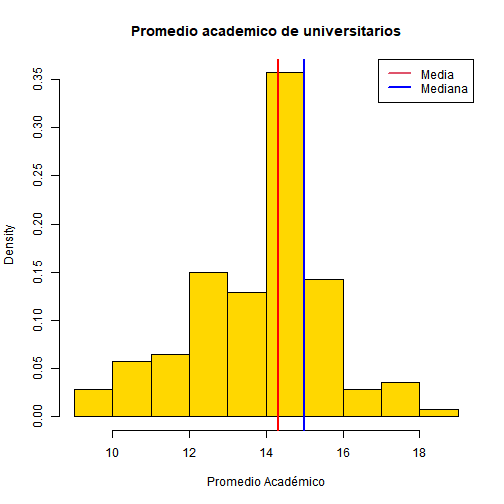
\includegraphics{S7_Infomre_E2_files/figure-latex/unnamed-chunk-9-1.pdf}
\textbf{Dispositivo que usa con mayor frecuencia}

``Falta agregar titulo''

\begin{Shaded}
\begin{Highlighting}[]
\NormalTok{Tabla }\OtherTok{\textless{}{-}}\NormalTok{ DFN}\SpecialCharTok{\%\textgreater{}\%} \FunctionTok{group\_by}\NormalTok{(Dispositivo) }\SpecialCharTok{\%\textgreater{}\%} \FunctionTok{summarise}\NormalTok{(}\AttributeTok{Total=}\FunctionTok{n}\NormalTok{())   }
    
\FunctionTok{ggplot}\NormalTok{(Tabla, }\FunctionTok{aes}\NormalTok{(}\AttributeTok{x =} \StringTok{"Dispositivos"}\NormalTok{, }\AttributeTok{y=}\NormalTok{Total,}\AttributeTok{fill=}\NormalTok{Dispositivo) ) }\SpecialCharTok{+}    
  \FunctionTok{geom\_bar}\NormalTok{(}\AttributeTok{width =} \FloatTok{0.9}\NormalTok{, }\AttributeTok{stat=}\StringTok{"identity"}\NormalTok{,              }
           \AttributeTok{position =} \FunctionTok{position\_dodge}\NormalTok{()                 )}\SpecialCharTok{+}  
  
  \FunctionTok{ylim}\NormalTok{(}\FunctionTok{c}\NormalTok{(}\DecValTok{0}\NormalTok{,}\DecValTok{125}\NormalTok{))}\SpecialCharTok{+}
  \FunctionTok{labs}\NormalTok{(}\AttributeTok{x=}\StringTok{"Dispositivos de los encuestados"}\NormalTok{, }\AttributeTok{y=} \StringTok{"Frecuencia"}\NormalTok{) }\SpecialCharTok{+}   
  \FunctionTok{labs}\NormalTok{(}\AttributeTok{fill =} \StringTok{""}\NormalTok{)}\SpecialCharTok{+}                                         
  
  \FunctionTok{geom\_text}\NormalTok{(}\FunctionTok{aes}\NormalTok{(}\AttributeTok{label=}\NormalTok{Total), }\AttributeTok{vjust=}\FloatTok{1.6}\NormalTok{, }\AttributeTok{color=}\StringTok{"black"}\NormalTok{,    }
              \AttributeTok{position =} \FunctionTok{position\_dodge}\NormalTok{(}\FloatTok{0.9}\NormalTok{),  }\AttributeTok{size=}\FloatTok{4.0}
\NormalTok{            ) }\SpecialCharTok{+}                                            
  
  \FunctionTok{theme\_bw}\NormalTok{(}\AttributeTok{base\_size =} \DecValTok{10}\NormalTok{)}
\end{Highlighting}
\end{Shaded}

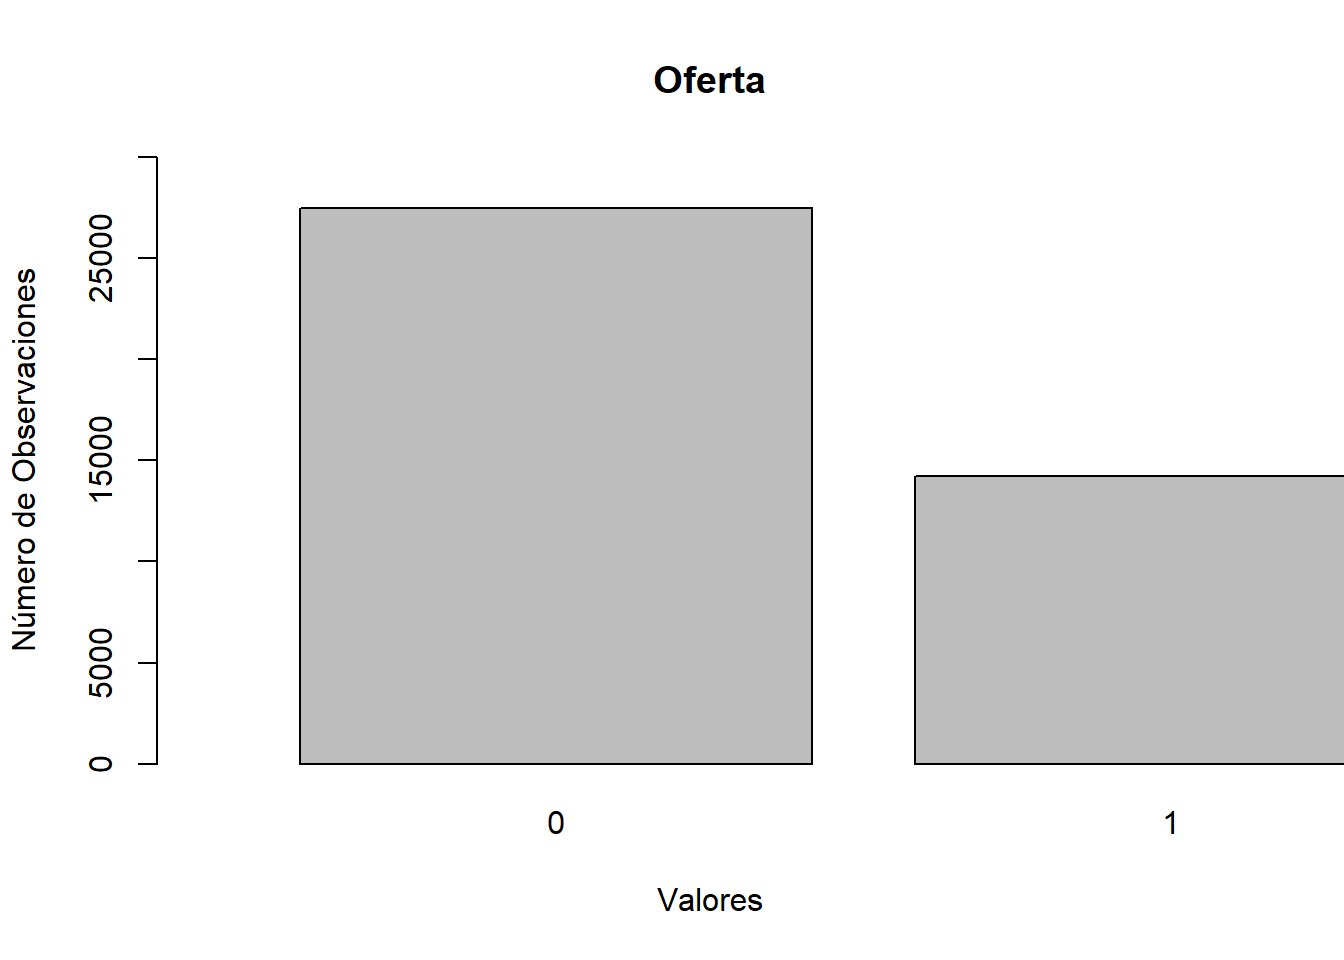
\includegraphics{S7_Infomre_E2_files/figure-latex/unnamed-chunk-10-1.pdf}

``Falta agregar titulo''

\begin{Shaded}
\begin{Highlighting}[]
\NormalTok{Tabla }\OtherTok{\textless{}{-}}\NormalTok{ DFN}\SpecialCharTok{\%\textgreater{}\%} \FunctionTok{group\_by}\NormalTok{(lugar\_uso) }\SpecialCharTok{\%\textgreater{}\%} \FunctionTok{summarise}\NormalTok{(}\AttributeTok{Total=}\FunctionTok{n}\NormalTok{())   }
    
\FunctionTok{ggplot}\NormalTok{(Tabla, }\FunctionTok{aes}\NormalTok{(}\AttributeTok{x =} \StringTok{"Lugar de uso"}\NormalTok{, }\AttributeTok{y=}\NormalTok{Total,}\AttributeTok{fill=}\NormalTok{lugar\_uso) ) }\SpecialCharTok{+}    
  \FunctionTok{geom\_bar}\NormalTok{(}\AttributeTok{width =} \FloatTok{0.9}\NormalTok{, }\AttributeTok{stat=}\StringTok{"identity"}\NormalTok{,              }
           \AttributeTok{position =} \FunctionTok{position\_dodge}\NormalTok{()                 )}\SpecialCharTok{+}  
  
  \FunctionTok{ylim}\NormalTok{(}\FunctionTok{c}\NormalTok{(}\DecValTok{0}\NormalTok{,}\DecValTok{40}\NormalTok{))}\SpecialCharTok{+}
  \FunctionTok{labs}\NormalTok{(}\AttributeTok{x=}\StringTok{"Dispositivos de los encuestados"}\NormalTok{, }\AttributeTok{y=} \StringTok{"Frecuencia"}\NormalTok{) }\SpecialCharTok{+}   
  \FunctionTok{labs}\NormalTok{(}\AttributeTok{fill =} \StringTok{""}\NormalTok{)}\SpecialCharTok{+}                                         
  
  \FunctionTok{geom\_text}\NormalTok{(}\FunctionTok{aes}\NormalTok{(}\AttributeTok{label=}\NormalTok{Total), }\AttributeTok{vjust=}\FloatTok{1.6}\NormalTok{, }\AttributeTok{color=}\StringTok{"black"}\NormalTok{,    }
              \AttributeTok{position =} \FunctionTok{position\_dodge}\NormalTok{(}\FloatTok{0.9}\NormalTok{),  }\AttributeTok{size=}\FloatTok{4.0}
\NormalTok{            ) }\SpecialCharTok{+}                                            
  
  \FunctionTok{theme\_bw}\NormalTok{(}\AttributeTok{base\_size =} \DecValTok{10}\NormalTok{)}
\end{Highlighting}
\end{Shaded}

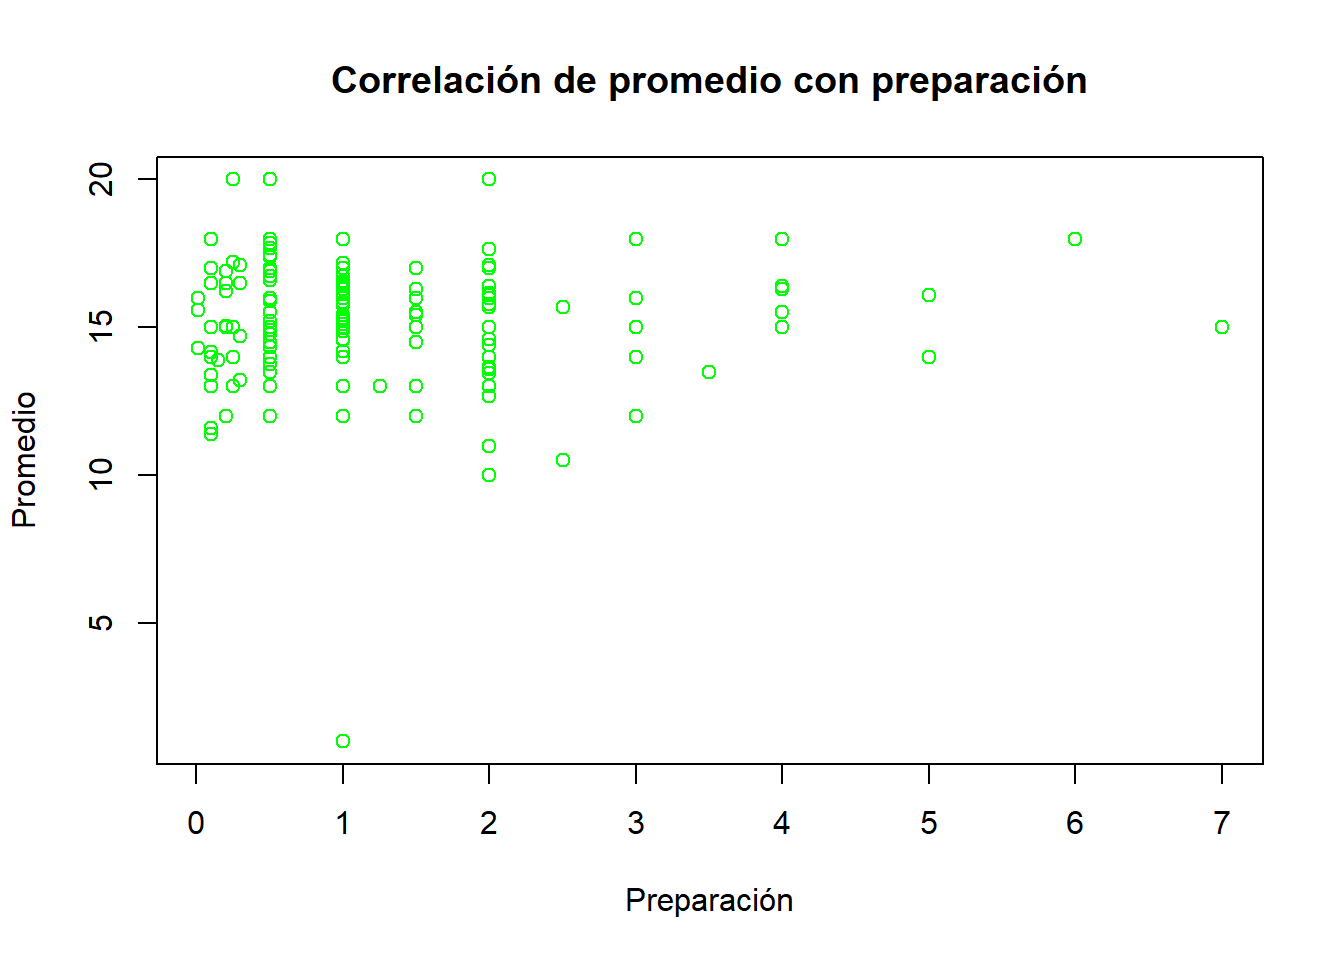
\includegraphics{S7_Infomre_E2_files/figure-latex/unnamed-chunk-11-1.pdf}

\hypertarget{grafico-mosaico}{%
\subsection{- Grafico Mosaico}\label{grafico-mosaico}}

\textbf{Categorico- Categorico}

\begin{Shaded}
\begin{Highlighting}[]
\FunctionTok{mosaicplot}\NormalTok{(DFN}\SpecialCharTok{$}\NormalTok{Angustia\_sin\_celular}\SpecialCharTok{\textasciitilde{}}\NormalTok{DFN}\SpecialCharTok{$}\NormalTok{Sexo,}\AttributeTok{col=}\FunctionTok{colorRampPalette}\NormalTok{(}\FunctionTok{c}\NormalTok{(}\StringTok{\textquotesingle{}white\textquotesingle{}}\NormalTok{,}\StringTok{\textquotesingle{}aquamarine4\textquotesingle{}}\NormalTok{))(}\DecValTok{4}\NormalTok{), }\AttributeTok{main=}\StringTok{"Género vs Angustia sin celular "}\NormalTok{,}\AttributeTok{xlab=}\StringTok{"Angustia sin celular"}\NormalTok{,}\AttributeTok{ylab=}\StringTok{"Género"}\NormalTok{)}
\FunctionTok{legend}\NormalTok{(}\AttributeTok{x =} \StringTok{"topright"}\NormalTok{, }\AttributeTok{legend =} \FunctionTok{c}\NormalTok{(}\StringTok{"Hombre"}\NormalTok{, }\StringTok{"Mujer"}\NormalTok{), }\AttributeTok{fill =}\FunctionTok{colorRampPalette}\NormalTok{(}\FunctionTok{c}\NormalTok{(}\StringTok{\textquotesingle{}white\textquotesingle{}}\NormalTok{,}\StringTok{\textquotesingle{}aquamarine4\textquotesingle{}}\NormalTok{))(}\DecValTok{5}\NormalTok{), }
       \AttributeTok{title =} \StringTok{"Leyenda"}\NormalTok{)}
\end{Highlighting}
\end{Shaded}

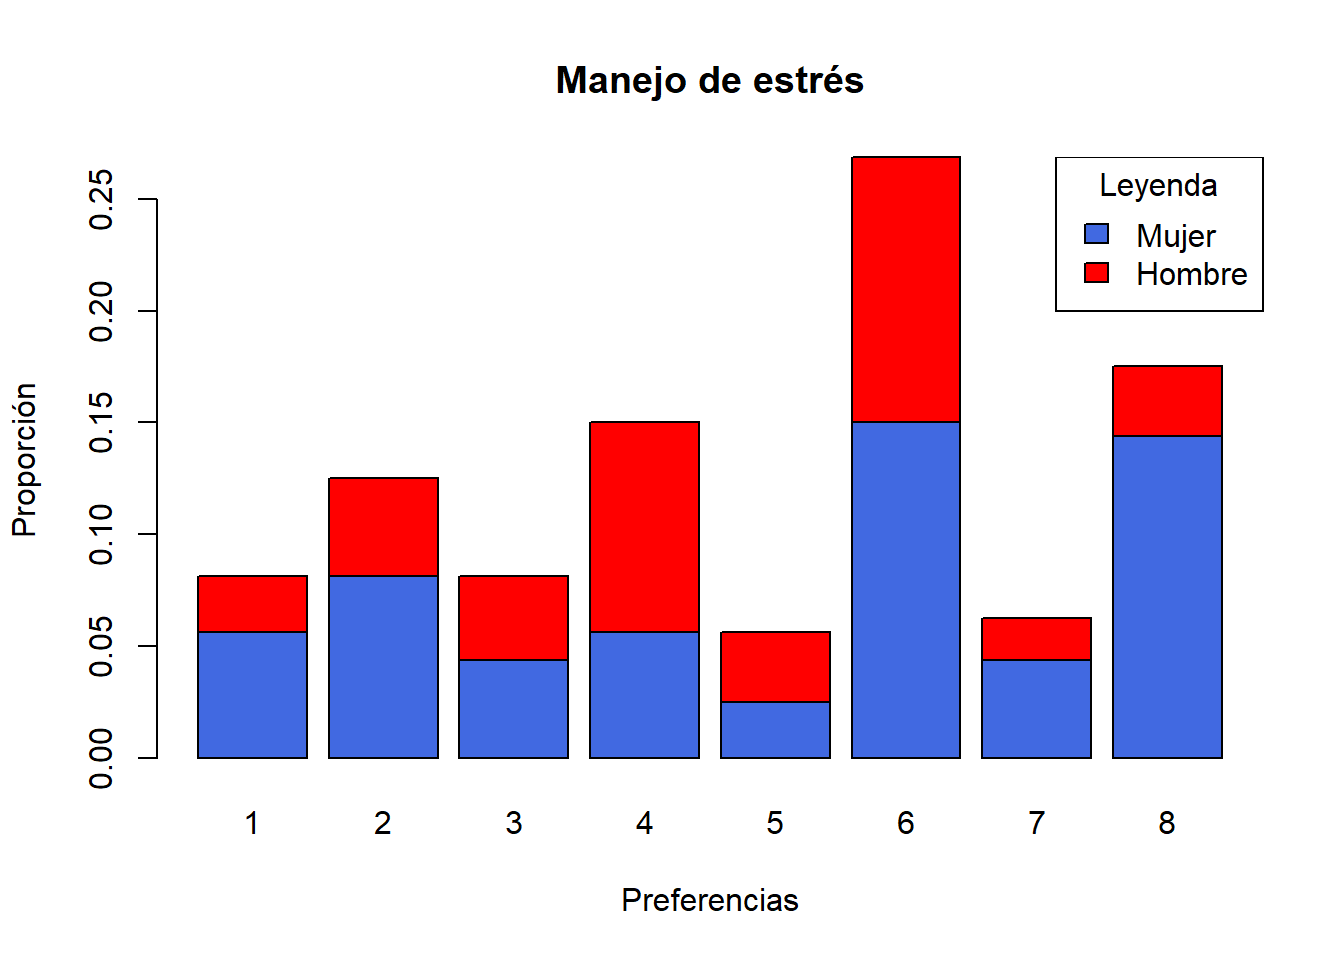
\includegraphics{S7_Infomre_E2_files/figure-latex/unnamed-chunk-12-1.pdf}

\begin{Shaded}
\begin{Highlighting}[]
\FunctionTok{mosaicplot}\NormalTok{(DFN}\SpecialCharTok{$}\NormalTok{Angustia\_bateria\_baja}\SpecialCharTok{\textasciitilde{}}\NormalTok{DFN}\SpecialCharTok{$}\NormalTok{Sexo,}\AttributeTok{col=}\FunctionTok{colorRampPalette}\NormalTok{(}\FunctionTok{c}\NormalTok{(}\StringTok{\textquotesingle{}white\textquotesingle{}}\NormalTok{,}\StringTok{\textquotesingle{}aquamarine4\textquotesingle{}}\NormalTok{))(}\DecValTok{4}\NormalTok{), }\AttributeTok{main=}\StringTok{"Género vs Angustia batería baja"}\NormalTok{,}\AttributeTok{xlab=}\StringTok{"Angustia sin batería del celular"}\NormalTok{,}\AttributeTok{ylab=}\StringTok{"Género"}\NormalTok{)}
\FunctionTok{legend}\NormalTok{(}\AttributeTok{x =} \StringTok{"topright"}\NormalTok{, }\AttributeTok{legend =} \FunctionTok{c}\NormalTok{(}\StringTok{"Hombre"}\NormalTok{, }\StringTok{"Mujer"}\NormalTok{), }\AttributeTok{fill =}\FunctionTok{colorRampPalette}\NormalTok{(}\FunctionTok{c}\NormalTok{(}\StringTok{\textquotesingle{}white\textquotesingle{}}\NormalTok{,}\StringTok{\textquotesingle{}aquamarine4\textquotesingle{}}\NormalTok{))(}\DecValTok{5}\NormalTok{), }
       \AttributeTok{title =} \StringTok{"Leyenda"}\NormalTok{)}
\end{Highlighting}
\end{Shaded}

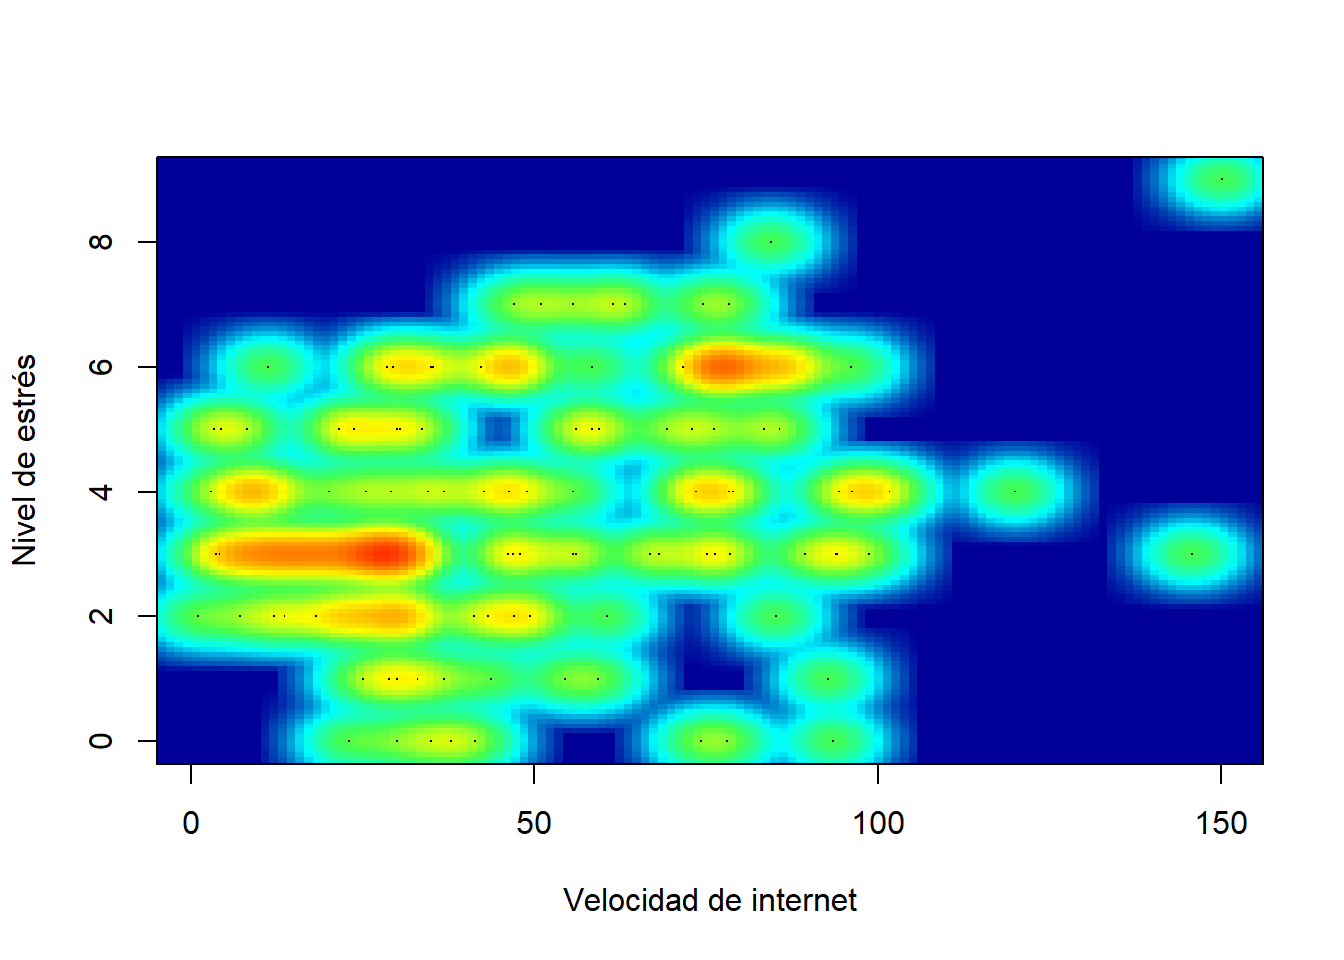
\includegraphics{S7_Infomre_E2_files/figure-latex/unnamed-chunk-13-1.pdf}

\hypertarget{grafico-histograma}{%
\subsection{- Grafico Histograma}\label{grafico-histograma}}

\begin{Shaded}
\begin{Highlighting}[]
\NormalTok{x }\OtherTok{\textless{}{-}}\NormalTok{ DFN}\SpecialCharTok{$}\NormalTok{Angustia\_sin\_celular}
\NormalTok{dx}\OtherTok{\textless{}{-}} \FunctionTok{density}\NormalTok{(x)}
\NormalTok{model}\OtherTok{\textless{}{-}}\FunctionTok{fitdist}\NormalTok{(x, }\StringTok{"gamma"}\NormalTok{)}
\NormalTok{a}\OtherTok{=}\NormalTok{model}\SpecialCharTok{$}\NormalTok{estimate[}\DecValTok{1}\NormalTok{]}
\NormalTok{b}\OtherTok{=}\NormalTok{model}\SpecialCharTok{$}\NormalTok{estimate[}\DecValTok{2}\NormalTok{]  }
\NormalTok{h}\OtherTok{\textless{}{-}}\FunctionTok{hist}\NormalTok{(DFN}\SpecialCharTok{$}\NormalTok{Angustia\_sin\_celular,}\AttributeTok{breaks=}\DecValTok{10}\NormalTok{, }\AttributeTok{freq=}\ConstantTok{FALSE}\NormalTok{, }\AttributeTok{main=}\StringTok{"Histograma de Angustia sin celular"}\NormalTok{, }\AttributeTok{ylab =} \StringTok{"Densidad"}\NormalTok{ ,}\AttributeTok{xlab=}\StringTok{"Nivel de Angustia "}\NormalTok{, }\AttributeTok{col=}\StringTok{"hotpink"}\NormalTok{)}
\FunctionTok{lines}\NormalTok{(dx, }\AttributeTok{lwd =} \DecValTok{2}\NormalTok{, }\AttributeTok{col =} \StringTok{"blue"}\NormalTok{)}
\FunctionTok{curve}\NormalTok{(}\FunctionTok{dgamma}\NormalTok{(x,a,b),}\AttributeTok{from=}\DecValTok{0}\NormalTok{,}\AttributeTok{to=}\DecValTok{100}\NormalTok{,}\AttributeTok{col=}\StringTok{"red"}\NormalTok{,}\AttributeTok{lwd=}\DecValTok{2}\NormalTok{,}\AttributeTok{add=}\NormalTok{T)}
\FunctionTok{legend}\NormalTok{(}\StringTok{"topright"}\NormalTok{, }\FunctionTok{c}\NormalTok{(}\StringTok{"curva observada"}\NormalTok{, }\StringTok{"curva (normal) teórica"}\NormalTok{),}
       \AttributeTok{lty =} \DecValTok{1}\NormalTok{, }\AttributeTok{lwd =} \DecValTok{2}\NormalTok{, }\AttributeTok{col =} \FunctionTok{c}\NormalTok{(}\StringTok{"red"}\NormalTok{, }\StringTok{"blue"}\NormalTok{), }\AttributeTok{bty =} \StringTok{"n"}\NormalTok{,}
       \AttributeTok{cex =} \FloatTok{0.8}\NormalTok{)}
\end{Highlighting}
\end{Shaded}

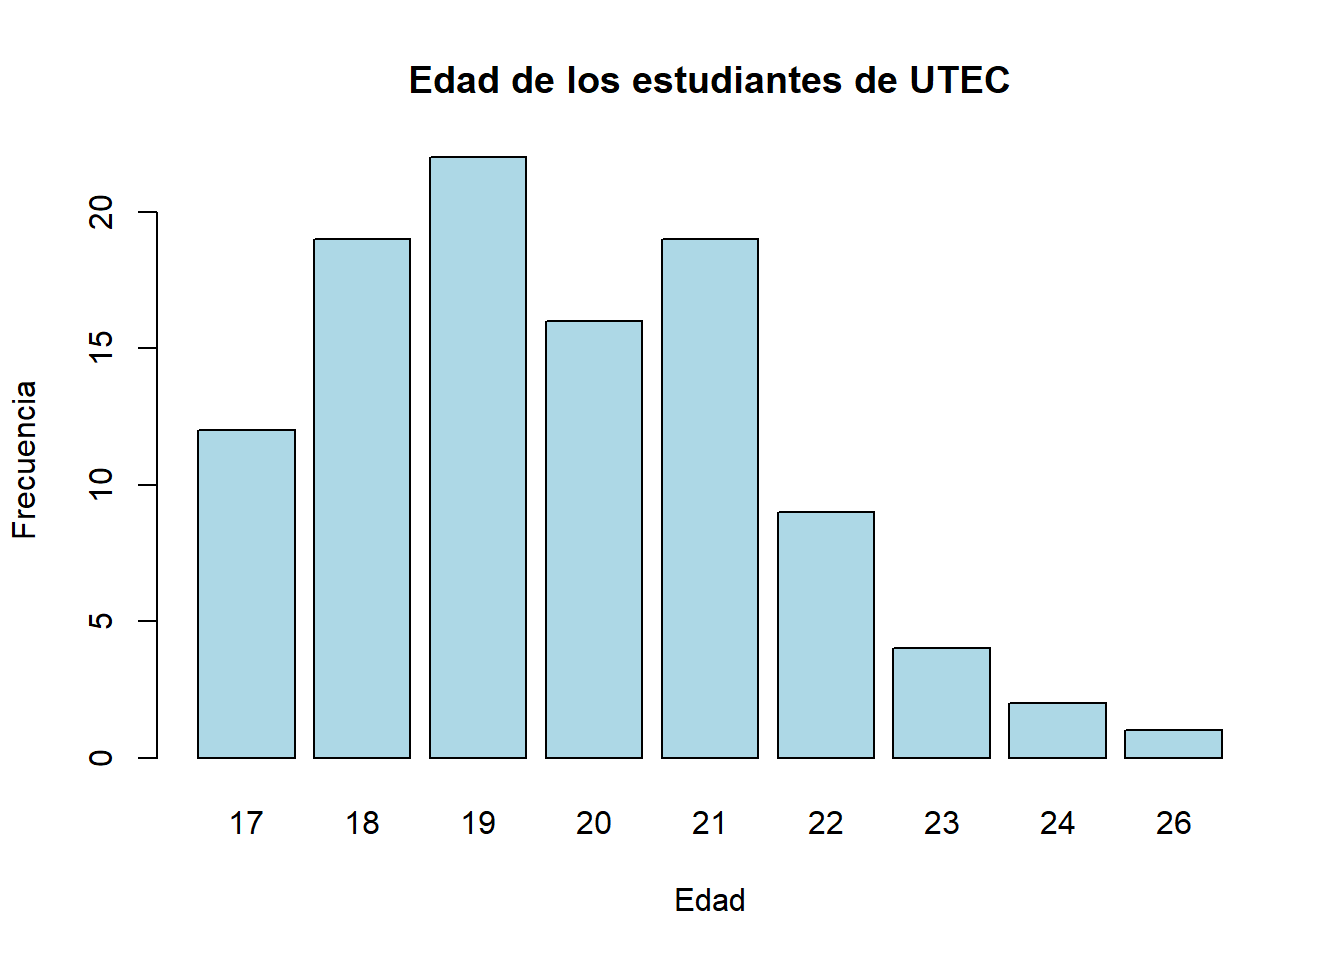
\includegraphics{S7_Infomre_E2_files/figure-latex/unnamed-chunk-14-1.pdf}

\hypertarget{histograma-de-edad}{%
\subsection{- Histograma de edad}\label{histograma-de-edad}}

\textbf{Es unimodal}

\begin{Shaded}
\begin{Highlighting}[]
\NormalTok{x }\OtherTok{\textless{}{-}}\NormalTok{ DFN}\SpecialCharTok{$}\NormalTok{Edad}
\NormalTok{dx}\OtherTok{\textless{}{-}} \FunctionTok{density}\NormalTok{(x)}
\NormalTok{model}\OtherTok{\textless{}{-}}\FunctionTok{fitdist}\NormalTok{(x, }\StringTok{"gamma"}\NormalTok{)}
\NormalTok{a}\OtherTok{=}\NormalTok{model}\SpecialCharTok{$}\NormalTok{estimate[}\DecValTok{1}\NormalTok{]}
\NormalTok{b}\OtherTok{=}\NormalTok{model}\SpecialCharTok{$}\NormalTok{estimate[}\DecValTok{2}\NormalTok{]  }
\NormalTok{h}\OtherTok{\textless{}{-}}\FunctionTok{hist}\NormalTok{(DFN}\SpecialCharTok{$}\NormalTok{Edad,}\AttributeTok{breaks=}\DecValTok{10}\NormalTok{, }\AttributeTok{freq=}\ConstantTok{FALSE}\NormalTok{, }\AttributeTok{main=}\StringTok{"Histograma de Edad"}\NormalTok{, }\AttributeTok{ylab =} \StringTok{"Densidad"}\NormalTok{ ,}\AttributeTok{xlab=}\StringTok{"Edad (en años) "}\NormalTok{, }\AttributeTok{col=}\StringTok{"hotpink"}\NormalTok{)}
\FunctionTok{lines}\NormalTok{(dx, }\AttributeTok{lwd =} \DecValTok{2}\NormalTok{, }\AttributeTok{col =} \StringTok{"blue"}\NormalTok{)}
\FunctionTok{curve}\NormalTok{(}\FunctionTok{dgamma}\NormalTok{(x,a,b),}\AttributeTok{from=}\DecValTok{0}\NormalTok{,}\AttributeTok{to=}\DecValTok{100}\NormalTok{,}\AttributeTok{col=}\StringTok{"red"}\NormalTok{,}\AttributeTok{lwd=}\DecValTok{2}\NormalTok{,}\AttributeTok{add=}\NormalTok{T)}
\FunctionTok{legend}\NormalTok{(}\StringTok{"topright"}\NormalTok{, }\FunctionTok{c}\NormalTok{(}\StringTok{"curva observada"}\NormalTok{, }\StringTok{"curva (normal) teórica"}\NormalTok{),}
       \AttributeTok{lty =} \DecValTok{1}\NormalTok{, }\AttributeTok{lwd =} \DecValTok{2}\NormalTok{, }\AttributeTok{col =} \FunctionTok{c}\NormalTok{(}\StringTok{"red"}\NormalTok{, }\StringTok{"blue"}\NormalTok{), }\AttributeTok{bty =} \StringTok{"n"}\NormalTok{,}
       \AttributeTok{cex =} \FloatTok{0.8}\NormalTok{)}
\end{Highlighting}
\end{Shaded}

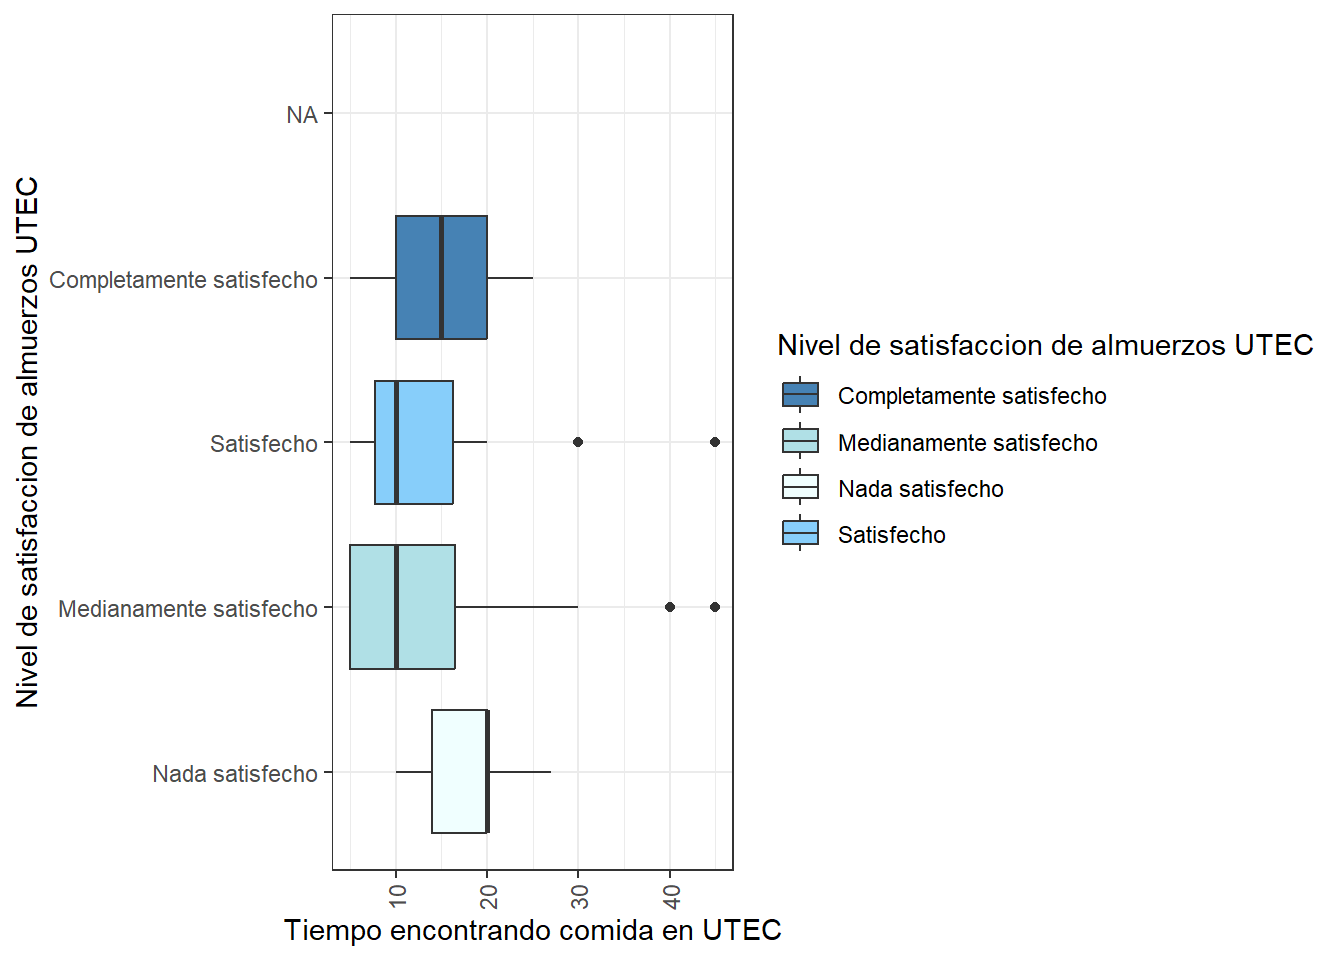
\includegraphics{S7_Infomre_E2_files/figure-latex/unnamed-chunk-15-1.pdf}
\#\#\#Histograma de edad del primer celular:

\textbf{Eliminar datos atipicos y rellenarlos con NA}

\begin{Shaded}
\begin{Highlighting}[]
\NormalTok{DFN}\SpecialCharTok{$}\NormalTok{Edad\_del\_primero\_celular [DFN}\SpecialCharTok{$}\NormalTok{Edad\_del\_primero\_celular}\SpecialCharTok{\textgreater{}}\DecValTok{20}\NormalTok{]}\OtherTok{\textless{}{-}} \ConstantTok{NA}
\FunctionTok{summary}\NormalTok{(DFN}\SpecialCharTok{$}\NormalTok{Edad\_del\_primero\_celular)}
\end{Highlighting}
\end{Shaded}

\begin{verbatim}
##    Min. 1st Qu.  Median    Mean 3rd Qu.    Max.    NA's 
##     5.0    11.0    13.0    12.8    15.0    19.0       2
\end{verbatim}

\begin{Shaded}
\begin{Highlighting}[]
\NormalTok{op}\OtherTok{=}\FunctionTok{par}\NormalTok{(}\AttributeTok{mfrow=}\FunctionTok{c}\NormalTok{(}\DecValTok{1}\NormalTok{,}\DecValTok{2}\NormalTok{))}

\CommentTok{\#{-}{-}{-}{-}{-}{-}{-}{-}{-}{-}{-}{-}{-}{-}{-}{-}{-}{-}{-}{-}{-}{-}{-}{-}{-}{-}{-}}

\FunctionTok{hist}\NormalTok{(DFN}\SpecialCharTok{$}\NormalTok{Edad\_del\_primero\_celular, }\AttributeTok{breaks=}\DecValTok{10}\NormalTok{, }\AttributeTok{freq =} \ConstantTok{FALSE}\NormalTok{, }\AttributeTok{main=}\StringTok{"Histograma del primer celular"}\NormalTok{,}\AttributeTok{xlab=}\StringTok{"Edad (años)"}\NormalTok{,}\AttributeTok{ylab =} \StringTok{"Densidad"}\NormalTok{, }\AttributeTok{col =} \StringTok{"lightblue"}\NormalTok{)}
\FunctionTok{curve}\NormalTok{(}\FunctionTok{dnorm}\NormalTok{(x, }\FunctionTok{mean}\NormalTok{(DFN}\SpecialCharTok{$}\NormalTok{Edad\_del\_primero\_celular,}\AttributeTok{na.rm =} \ConstantTok{TRUE}\NormalTok{), }\AttributeTok{sd =} \FunctionTok{sd}\NormalTok{(DFN}\SpecialCharTok{$}\NormalTok{Edad\_del\_primero\_celular,}\AttributeTok{na.rm =} \ConstantTok{TRUE}\NormalTok{)), }\CommentTok{\# Función dnorm a evaluar}
      \DecValTok{0}\NormalTok{, }\DecValTok{300}\NormalTok{, }\DecValTok{40}\NormalTok{, }\CommentTok{\# Límites de x y nº de valores a evaluar}
      \AttributeTok{col =} \StringTok{"red"}\NormalTok{, }
      \AttributeTok{las =} \DecValTok{1}\NormalTok{, }\CommentTok{\# Etiquetas alineadas horizontalmente}
      \AttributeTok{ann =} \ConstantTok{FALSE}\NormalTok{, }\CommentTok{\# Sin títulos en los ejes}
      \AttributeTok{xaxp =} \FunctionTok{c}\NormalTok{(}\DecValTok{0}\NormalTok{, }\DecValTok{300}\NormalTok{, }\DecValTok{10}\NormalTok{),  }\CommentTok{\# Marcas del eje x}
      \AttributeTok{ylim =} \FunctionTok{c}\NormalTok{(}\DecValTok{0}\NormalTok{,}\FloatTok{0.03}\NormalTok{), }\CommentTok{\# Límites del eje}
      \AttributeTok{yaxs =} \StringTok{"i"}\NormalTok{, }\AttributeTok{add =} \ConstantTok{TRUE}\NormalTok{) }\CommentTok{\# Estilo del eje y, ajustado a los límites}
\FunctionTok{points}\NormalTok{(DFN}\SpecialCharTok{$}\NormalTok{Edad\_del\_primero\_celular, }\FunctionTok{dnorm}\NormalTok{(DFN}\SpecialCharTok{$}\NormalTok{Edad\_del\_primero\_celular, }\FunctionTok{mean}\NormalTok{(DFN}\SpecialCharTok{$}\NormalTok{Edad\_del\_primero\_celular,}\AttributeTok{na.rm =} \ConstantTok{TRUE}\NormalTok{), }\AttributeTok{sd =} \FunctionTok{sd}\NormalTok{(DFN}\SpecialCharTok{$}\NormalTok{Edad\_del\_primero\_celular,}\AttributeTok{na.rm =} \ConstantTok{TRUE}\NormalTok{)), }\AttributeTok{ylab =} \StringTok{"f(x)"}\NormalTok{, }\AttributeTok{pch =} \DecValTok{20}\NormalTok{,  }\AttributeTok{lwd =} \FloatTok{0.1}\NormalTok{, }\AttributeTok{col =} \StringTok{"navyblue"}\NormalTok{)}
\FunctionTok{par}\NormalTok{(op)}
\end{Highlighting}
\end{Shaded}

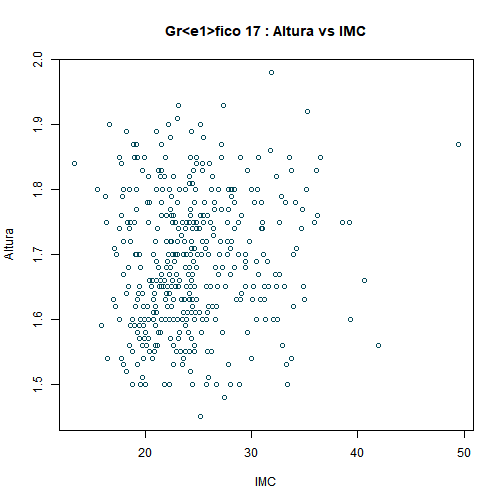
\includegraphics[width=0.9\linewidth]{S7_Infomre_E2_files/figure-latex/unnamed-chunk-17-1}

\hypertarget{grafica-de-baxplots}{%
\subsection{- Grafica de BaxPlots}\label{grafica-de-baxplots}}

\textbf{Descriptor gráfico numerico - categorico}

\begin{Shaded}
\begin{Highlighting}[]
\FunctionTok{boxplot}\NormalTok{(DFN}\SpecialCharTok{$}\NormalTok{Tiempo\_de\_carga}\SpecialCharTok{\textasciitilde{}}\NormalTok{ DFN}\SpecialCharTok{$}\NormalTok{Angustia\_sin\_celular, }\AttributeTok{ylab =} \StringTok{"Tiempo de carga de batería"}\NormalTok{, }\AttributeTok{xlab =} \StringTok{"Nivel de angustia sin celular"}\NormalTok{, }\AttributeTok{col =}\FunctionTok{colorRampPalette}\NormalTok{(}\FunctionTok{c}\NormalTok{(}\StringTok{\textquotesingle{}orange\textquotesingle{}}\NormalTok{,}\StringTok{\textquotesingle{}aquamarine4\textquotesingle{}}\NormalTok{))(}\DecValTok{5}\NormalTok{),}\AttributeTok{main=}\StringTok{"Tiempo de carga de celular vs Nivel de angustia sin celular"}\NormalTok{)}
\FunctionTok{legend}\NormalTok{(}\AttributeTok{x =} \StringTok{"topright"}\NormalTok{, }\AttributeTok{legend =} \FunctionTok{c}\NormalTok{(}\StringTok{"1"}\NormalTok{, }\StringTok{"2"}\NormalTok{,}\StringTok{"3"}\NormalTok{,}\StringTok{"4"}\NormalTok{,}\StringTok{"5"}\NormalTok{), }\AttributeTok{fill =}\FunctionTok{colorRampPalette}\NormalTok{(}\FunctionTok{c}\NormalTok{(}\StringTok{\textquotesingle{}orange\textquotesingle{}}\NormalTok{,}\StringTok{\textquotesingle{}aquamarine4\textquotesingle{}}\NormalTok{))(}\DecValTok{5}\NormalTok{), }
       \AttributeTok{title =} \StringTok{"Leyenda"}\NormalTok{)}
\end{Highlighting}
\end{Shaded}

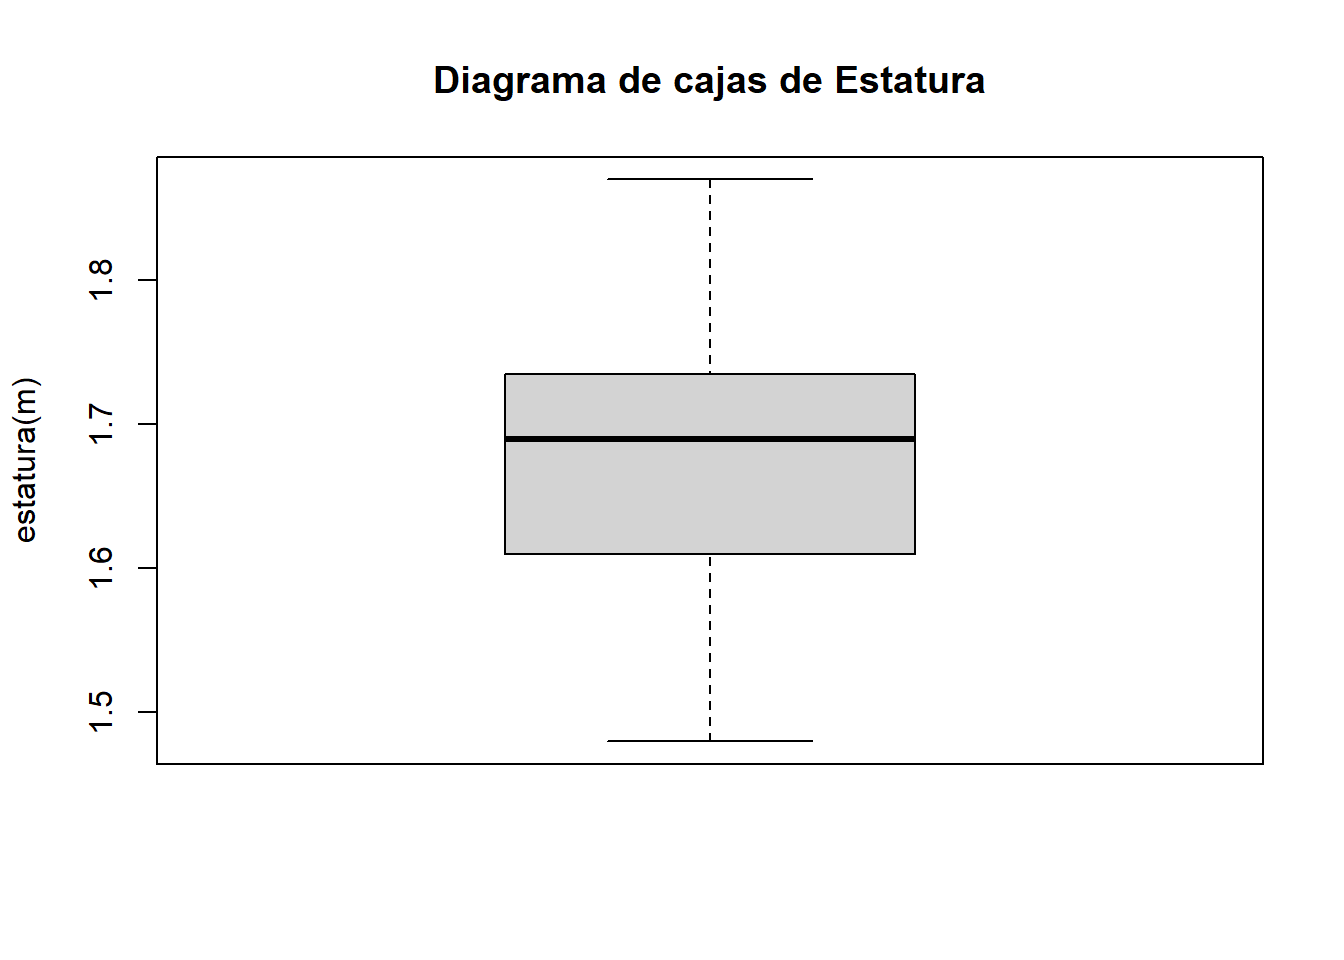
\includegraphics{S7_Infomre_E2_files/figure-latex/unnamed-chunk-18-1.pdf}

\hypertarget{grafica-de-dispersion}{%
\subsection{- Grafica de dispersion}\label{grafica-de-dispersion}}

\textbf{Para cada variable a analizar se debe de hacer esto
\emph{observación} }

\begin{Shaded}
\begin{Highlighting}[]
\FunctionTok{range}\NormalTok{(DFN}\SpecialCharTok{$}\NormalTok{Redes\_sociales, }\AttributeTok{na.rm=}\ConstantTok{TRUE}\NormalTok{)                            }\CommentTok{\#Rango }
\end{Highlighting}
\end{Shaded}

\begin{verbatim}
## [1]  20 500
\end{verbatim}

\begin{Shaded}
\begin{Highlighting}[]
\CommentTok{\# En promedio, la altura de los individuos encuestados el valor de 142 centímetros como mínimo y 182 centímetros como máximo, resultando 40 como rango absoluto.}
\FunctionTok{max}\NormalTok{(DFN}\SpecialCharTok{$}\NormalTok{Redes\_sociales, }\AttributeTok{na.rm=}\ConstantTok{TRUE}\NormalTok{)}\SpecialCharTok{{-}}\FunctionTok{min}\NormalTok{(DFN}\SpecialCharTok{$}\NormalTok{Redes\_sociales )        }\CommentTok{\#RANGO ABSOLUTO}
\end{Highlighting}
\end{Shaded}

\begin{verbatim}
## [1] 480
\end{verbatim}

\begin{Shaded}
\begin{Highlighting}[]
\FunctionTok{round}\NormalTok{(}\FunctionTok{var}\NormalTok{(DFN}\SpecialCharTok{$}\NormalTok{Redes\_sociales, }\AttributeTok{na.rm=}\ConstantTok{TRUE}\NormalTok{))                       }\CommentTok{\#VARIANZA}
\end{Highlighting}
\end{Shaded}

\begin{verbatim}
## [1] 6835
\end{verbatim}

\begin{Shaded}
\begin{Highlighting}[]
\CommentTok{\# El valor de la varianza para esta variable es de 48, que está muy por debajo de la media que es de 162,  esto se interpreta como que la dispersión de los datos es menor.}

\FunctionTok{round}\NormalTok{(}\FunctionTok{sd}\NormalTok{(DFN}\SpecialCharTok{$}\NormalTok{Redes\_sociales, }\AttributeTok{na.rm=}\ConstantTok{TRUE}\NormalTok{),}\AttributeTok{digits=}\DecValTok{2}\NormalTok{)               }\CommentTok{\#DESVIACIÓN ESTANDAR}
\end{Highlighting}
\end{Shaded}

\begin{verbatim}
## [1] 82.67
\end{verbatim}

\begin{Shaded}
\begin{Highlighting}[]
\CommentTok{\# El valor de la desviación estándar para esta variable es 6,85, entonces la variabilidad de las alturas es moderado.}

\NormalTok{cv }\OtherTok{\textless{}{-}}\NormalTok{(}\FunctionTok{sd}\NormalTok{(DFN}\SpecialCharTok{$}\NormalTok{Redes\_sociales, }\AttributeTok{na.rm =} \ConstantTok{TRUE}\NormalTok{)}\SpecialCharTok{/}\FunctionTok{mean}\NormalTok{(DFN}\SpecialCharTok{$}\NormalTok{Redes\_sociales, }\AttributeTok{na.rm =} \ConstantTok{TRUE}\NormalTok{))}\CommentTok{\# Coeficiente de variación}
\FunctionTok{round}\NormalTok{(cv,}\AttributeTok{digits =} \DecValTok{2}\NormalTok{)}
\end{Highlighting}
\end{Shaded}

\begin{verbatim}
## [1] 0.66
\end{verbatim}

\begin{Shaded}
\begin{Highlighting}[]
\CommentTok{\# Su coeficiente de variación es 0.04, existe mayor homogeneidad en los datos y tenemos una muestra compacta}
\end{Highlighting}
\end{Shaded}

\begin{Shaded}
\begin{Highlighting}[]
\FunctionTok{round}\NormalTok{(}\FunctionTok{cov}\NormalTok{(DFN}\SpecialCharTok{$}\NormalTok{Edad,DFN}\SpecialCharTok{$}\NormalTok{Angustia\_sin\_celular),}\AttributeTok{digits =} \DecValTok{2}\NormalTok{)}
\end{Highlighting}
\end{Shaded}

\begin{verbatim}
## [1] -0.41
\end{verbatim}

\begin{Shaded}
\begin{Highlighting}[]
\FunctionTok{round}\NormalTok{(}\FunctionTok{cor}\NormalTok{(DFN}\SpecialCharTok{$}\NormalTok{Edad,DFN}\SpecialCharTok{$}\NormalTok{Angustia\_sin\_celular),}\AttributeTok{digits =} \DecValTok{2}\NormalTok{)}
\end{Highlighting}
\end{Shaded}

\begin{verbatim}
## [1] -0.14
\end{verbatim}

``buscar mas informacion''

\hypertarget{cov.-negativa-relacion-debil-pero-negativa}{%
\subsection{-cov. negativa -- Relacion debil pero
negativa}\label{cov.-negativa-relacion-debil-pero-negativa}}

\emph{Numerico - Numerico}

\begin{Shaded}
\begin{Highlighting}[]
\FunctionTok{smoothScatter}\NormalTok{(DFN}\SpecialCharTok{$}\NormalTok{Redes\_sociales, DFN}\SpecialCharTok{$}\NormalTok{Uso\_del\_celular\_dia,  }\AttributeTok{xlab =} \StringTok{"Uso del celular al dia"}\NormalTok{, }\AttributeTok{ylab =} \StringTok{"Redes sociales"}\NormalTok{)}
\NormalTok{modelo1 }\OtherTok{\textless{}{-}} \FunctionTok{lm}\NormalTok{(DFN}\SpecialCharTok{$}\NormalTok{Uso\_del\_celular\_dia }\SpecialCharTok{\textasciitilde{}}\NormalTok{ DFN}\SpecialCharTok{$}\NormalTok{Redes\_sociales)}
\FunctionTok{abline}\NormalTok{(modelo1, }\AttributeTok{col =} \StringTok{"red"}\NormalTok{, }\AttributeTok{lwd =} \DecValTok{2}\NormalTok{)}
\end{Highlighting}
\end{Shaded}

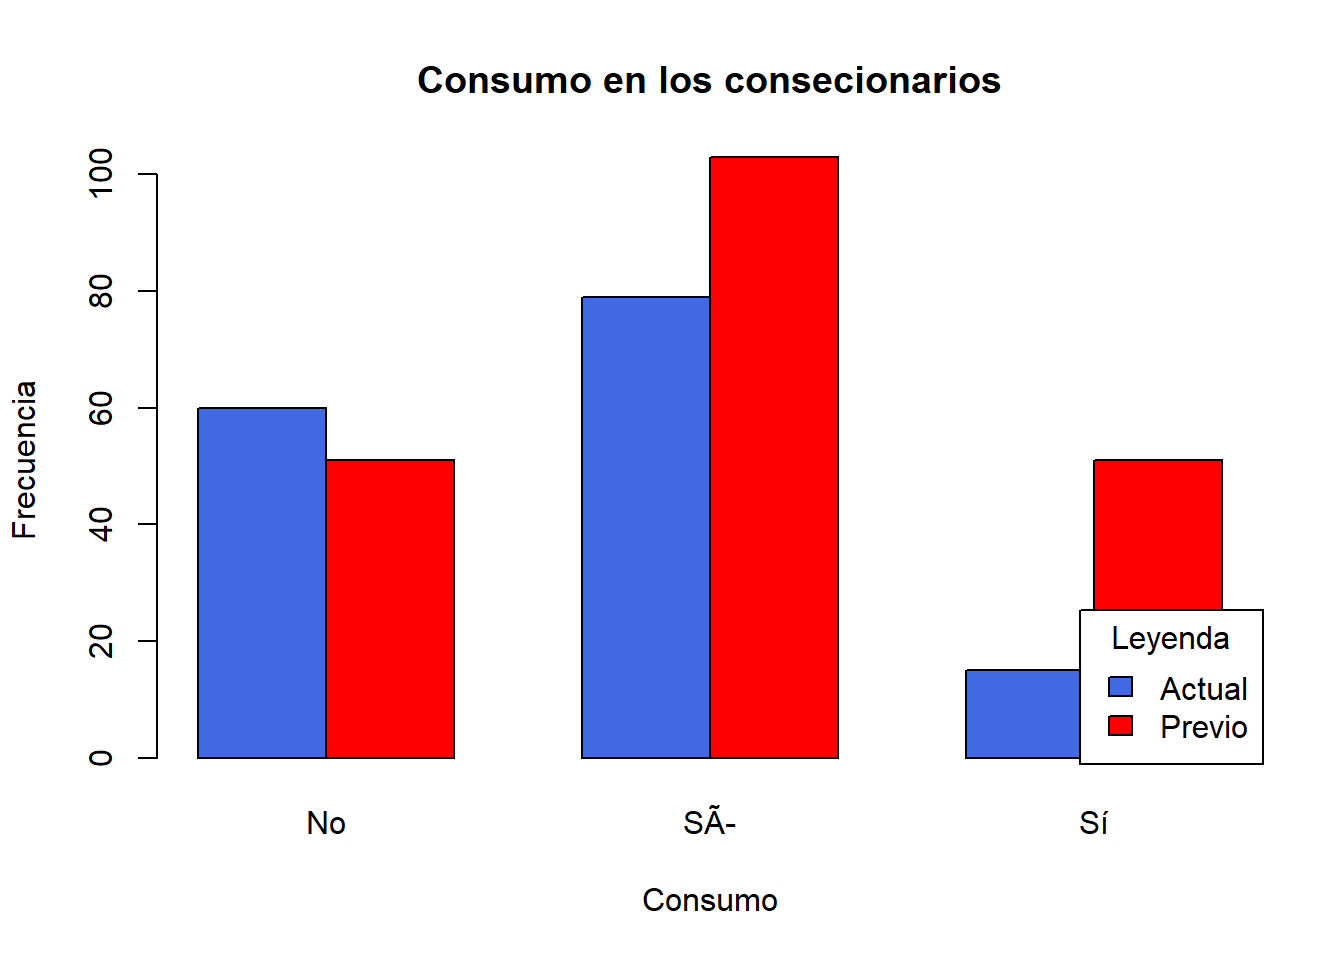
\includegraphics{S7_Infomre_E2_files/figure-latex/unnamed-chunk-21-1.pdf}

\hypertarget{mayor-uso---mas-tiempo-en-el-cel}{%
\section{Mayor uso - Mas tiempo en el
cel}\label{mayor-uso---mas-tiempo-en-el-cel}}

\hypertarget{modelo-normal}{%
\subsection{-Modelo normal}\label{modelo-normal}}

\begin{Shaded}
\begin{Highlighting}[]
\NormalTok{Descrip}\OtherTok{\textless{}{-}}\ControlFlowTok{function}\NormalTok{(X)\{}
  \FunctionTok{return}\NormalTok{(}\FunctionTok{list}\NormalTok{(}\StringTok{\textquotesingle{}Media  \textquotesingle{}}\OtherTok{=}\FunctionTok{round}\NormalTok{(}\FunctionTok{mean}\NormalTok{(X,}\AttributeTok{na.rm =} \ConstantTok{TRUE}\NormalTok{ ),}\DecValTok{2}\NormalTok{), }\StringTok{\textquotesingle{}Mediana   \textquotesingle{}}\OtherTok{=}\FunctionTok{round}\NormalTok{(}\FunctionTok{median}\NormalTok{(X, }\AttributeTok{na.rm =} \ConstantTok{TRUE}\NormalTok{),}\DecValTok{2}\NormalTok{), }\StringTok{\textquotesingle{}Moda    \textquotesingle{}}\OtherTok{=}\FunctionTok{as.numeric}\NormalTok{(}\FunctionTok{names}\NormalTok{(}\FunctionTok{which}\NormalTok{(}\FunctionTok{table}\NormalTok{(X)}\SpecialCharTok{==}\FunctionTok{max}\NormalTok{(}\FunctionTok{table}\NormalTok{(X)))))))\}}
\end{Highlighting}
\end{Shaded}

\begin{Shaded}
\begin{Highlighting}[]
\FunctionTok{mapply}\NormalTok{(Descrip, }\FunctionTok{list}\NormalTok{(}\StringTok{\textquotesingle{}Edad del primer celular  \textquotesingle{}}\OtherTok{=}\NormalTok{DFN}\SpecialCharTok{$}\NormalTok{Edad\_del\_primero\_celular))}
\end{Highlighting}
\end{Shaded}

\begin{verbatim}
##            Edad del primer celular  
## Media      12.8                     
## Mediana    13                       
## Moda       15
\end{verbatim}

\hypertarget{limpieza-de-datos-atipicos}{%
\subsection{-Limpieza de datos
atipicos}\label{limpieza-de-datos-atipicos}}

\begin{Shaded}
\begin{Highlighting}[]
\NormalTok{DFN}\SpecialCharTok{$}\NormalTok{Edad\_del\_primero\_celular[DFN}\SpecialCharTok{$}\NormalTok{Edad\_del\_primero\_celular }\SpecialCharTok{==} \DecValTok{25}\NormalTok{]}\OtherTok{\textless{}{-}} \ConstantTok{NA}
\NormalTok{DFN}\SpecialCharTok{$}\NormalTok{Edad\_del\_primero\_celular[DFN}\SpecialCharTok{$}\NormalTok{Edad\_del\_primero\_celular }\SpecialCharTok{==} \DecValTok{6}\NormalTok{]}\OtherTok{\textless{}{-}} \ConstantTok{NA}
\NormalTok{DFN}\SpecialCharTok{$}\NormalTok{Edad\_del\_primero\_celular[DFN}\SpecialCharTok{$}\NormalTok{Edad\_del\_primero\_celular }\SpecialCharTok{==} \DecValTok{5}\NormalTok{]}\OtherTok{\textless{}{-}} \ConstantTok{NA}
\end{Highlighting}
\end{Shaded}

\begin{Shaded}
\begin{Highlighting}[]
\NormalTok{op}\OtherTok{=}\FunctionTok{par}\NormalTok{(}\AttributeTok{mfrow=}\FunctionTok{c}\NormalTok{(}\DecValTok{1}\NormalTok{,}\DecValTok{2}\NormalTok{))}

\CommentTok{\#{-}{-}{-}{-}{-}{-}{-}{-}{-}{-}{-}{-}{-}{-}{-}{-}{-}{-}{-}{-}{-}{-}{-}{-}{-}{-}{-}}

\FunctionTok{hist}\NormalTok{(DFN}\SpecialCharTok{$}\NormalTok{Edad\_del\_primero\_celular, }\AttributeTok{breaks=}\DecValTok{10}\NormalTok{, }\AttributeTok{freq =} \ConstantTok{FALSE}\NormalTok{, }\AttributeTok{main=}\StringTok{"Histograma del año del primer celular"}\NormalTok{,}\AttributeTok{xlab=}\StringTok{"Edad"}\NormalTok{,}\AttributeTok{ylab =} \StringTok{"Densidad"}\NormalTok{, }\AttributeTok{col =} \StringTok{"lightblue"}\NormalTok{)}
\FunctionTok{curve}\NormalTok{(}\FunctionTok{dnorm}\NormalTok{(x, }\FunctionTok{mean}\NormalTok{(DFN}\SpecialCharTok{$}\NormalTok{Edad\_del\_primero\_celular,}\AttributeTok{na.rm =} \ConstantTok{TRUE}\NormalTok{), }\AttributeTok{sd =} \FunctionTok{sd}\NormalTok{(DFN}\SpecialCharTok{$}\NormalTok{Edad\_del\_primero\_celular,}\AttributeTok{na.rm =} \ConstantTok{TRUE}\NormalTok{)), }\CommentTok{\# Función dnorm a evaluar}
      \DecValTok{0}\NormalTok{, }\DecValTok{300}\NormalTok{, }\DecValTok{40}\NormalTok{, }\CommentTok{\# Límites de x y nº de valores a evaluar}
      \AttributeTok{col =} \StringTok{"red"}\NormalTok{, }
      \AttributeTok{las =} \DecValTok{1}\NormalTok{, }\CommentTok{\# Etiquetas alineadas horizontalmente}
      \AttributeTok{ann =} \ConstantTok{FALSE}\NormalTok{, }\CommentTok{\# Sin títulos en los ejes}
      \AttributeTok{xaxp =} \FunctionTok{c}\NormalTok{(}\DecValTok{0}\NormalTok{, }\DecValTok{300}\NormalTok{, }\DecValTok{10}\NormalTok{),  }\CommentTok{\# Marcas del eje x}
      \AttributeTok{ylim =} \FunctionTok{c}\NormalTok{(}\DecValTok{0}\NormalTok{,}\FloatTok{0.03}\NormalTok{), }\CommentTok{\# Límites del eje}
      \AttributeTok{yaxs =} \StringTok{"i"}\NormalTok{, }\AttributeTok{add =} \ConstantTok{TRUE}\NormalTok{) }\CommentTok{\# Estilo del eje y, ajustado a los límites}
\FunctionTok{points}\NormalTok{(DFN}\SpecialCharTok{$}\NormalTok{Edad\_del\_primero\_celular, }\FunctionTok{dnorm}\NormalTok{(DFN}\SpecialCharTok{$}\NormalTok{Edad\_del\_primero\_celular, }\FunctionTok{mean}\NormalTok{(DFN}\SpecialCharTok{$}\NormalTok{Edad\_del\_primero\_celular,}\AttributeTok{na.rm =} \ConstantTok{TRUE}\NormalTok{), }\AttributeTok{sd =} \FunctionTok{sd}\NormalTok{(DFN}\SpecialCharTok{$}\NormalTok{Edad\_del\_primero\_celular,}\AttributeTok{na.rm =} \ConstantTok{TRUE}\NormalTok{)), }\AttributeTok{ylab =} \StringTok{"f(x)"}\NormalTok{, }\AttributeTok{pch =} \DecValTok{20}\NormalTok{,  }\AttributeTok{lwd =} \FloatTok{0.1}\NormalTok{, }\AttributeTok{col =} \StringTok{"navyblue"}\NormalTok{)}
\FunctionTok{par}\NormalTok{(op)}
\end{Highlighting}
\end{Shaded}

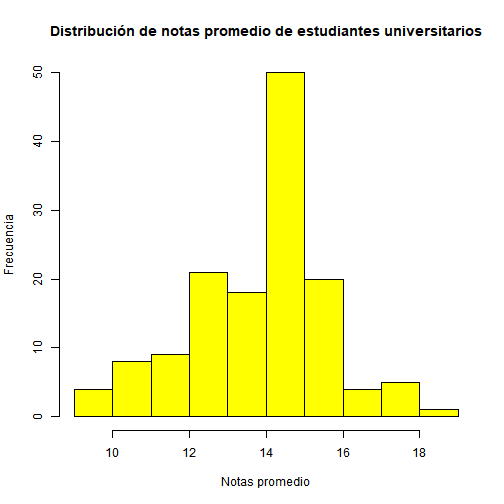
\includegraphics[width=0.9\linewidth]{S7_Infomre_E2_files/figure-latex/unnamed-chunk-25-1}

\hypertarget{analisis-probabilistico}{%
\subsection{-Analisis probabilistico}\label{analisis-probabilistico}}

Se tiene una población de 202 encuestados para considerar su tiempo en
redes sociales, debe estar conectado en redes sociales más de 240
minutos y se le considera bajo si la medida es menor. Si se toma una
encuesta de 40 encuestados, calcular la probabilidad de que todos en
esta muestra estén mas de 240 minutos en redes sociales. Se sabe que
existe 20 encuestados son considerados que se encuentran mas tiempo en
redes sociales.

\begin{Shaded}
\begin{Highlighting}[]
\NormalTok{x}\OtherTok{=}\DecValTok{40}
\NormalTok{M}\OtherTok{=}\DecValTok{202{-}20}
\NormalTok{N}\OtherTok{=}\DecValTok{202}
\NormalTok{n}\OtherTok{=}\DecValTok{40}

\FunctionTok{plot}\NormalTok{(}\FunctionTok{dhyper}\NormalTok{(x, }\DecValTok{40}\SpecialCharTok{:}\NormalTok{M, N}\SpecialCharTok{{-}}\NormalTok{M, n),}\AttributeTok{col =} \StringTok{"cadetblue3"}\NormalTok{,}\AttributeTok{xlab =} \StringTok{"Tiempo en redes sociales (min)"}\NormalTok{,}\AttributeTok{ylab =} \StringTok{"Probabilidad Hipergeométrica"}\NormalTok{,}\AttributeTok{main =} \StringTok{"MODELO HIPERGEOMÉTRICO {-} Tiempo en redes sociales "}\NormalTok{)}
\end{Highlighting}
\end{Shaded}

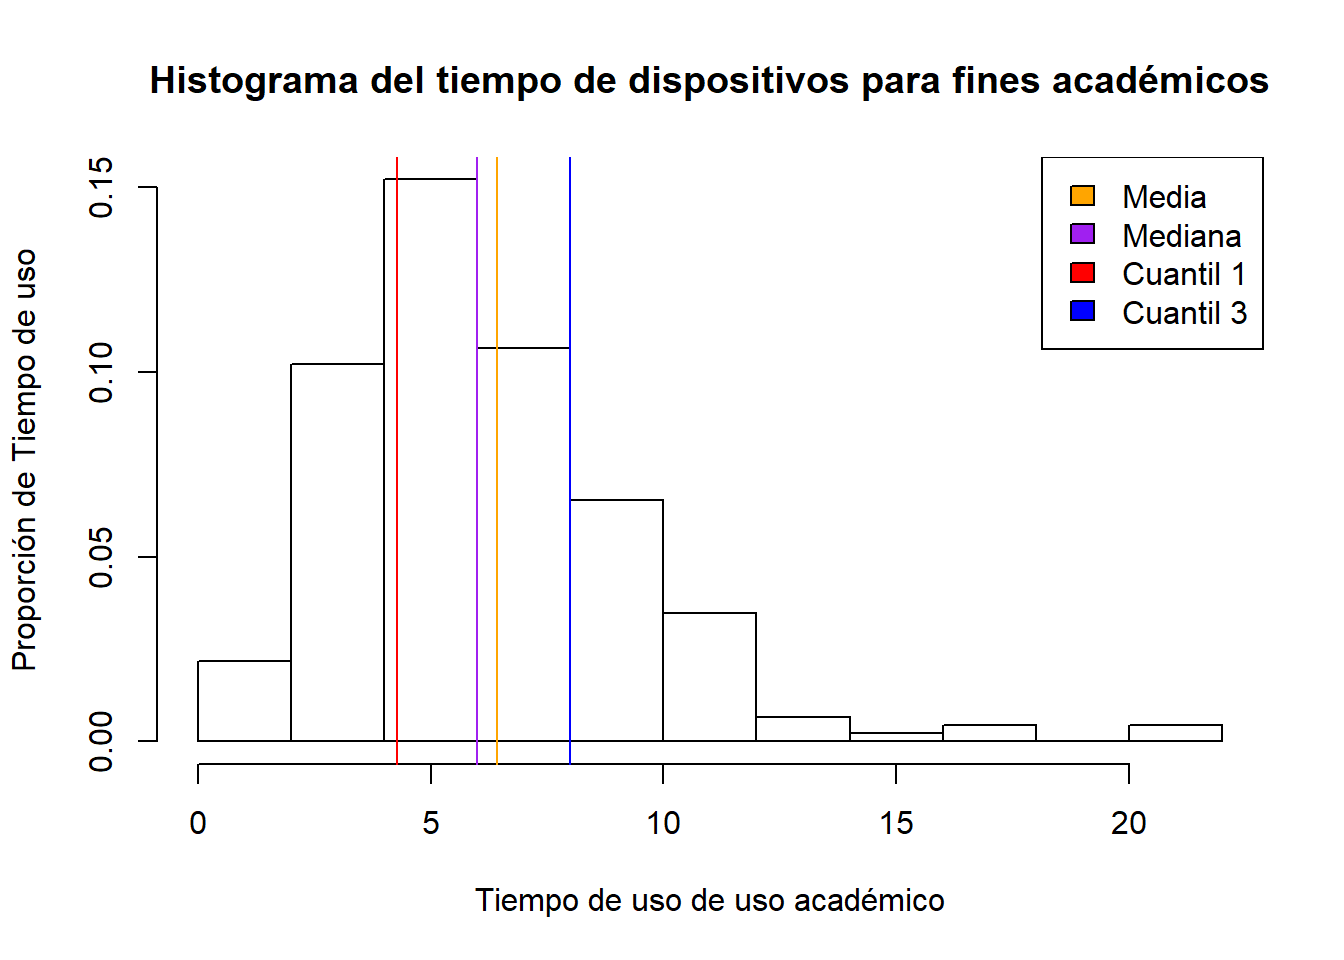
\includegraphics{S7_Infomre_E2_files/figure-latex/unnamed-chunk-26-1.pdf}

``buscar informacion''

\hypertarget{modelo-binomial}{%
\subsection{-Modelo Binomial}\label{modelo-binomial}}

Se sabe 80 de nuestros encuestados la probabilidad de un 20/202 de dejar
su celular cargando por 100 minutos. Si de 80 encuestados tomamos 3
personas. Calcular la probabilidad de que estas 3 personas carguen su
celular por 100 minutos.

\begin{Shaded}
\begin{Highlighting}[]
\NormalTok{n}\OtherTok{=}\DecValTok{3}
\NormalTok{k}\OtherTok{=}\DecValTok{80}
\NormalTok{p}\OtherTok{=}\DecValTok{20}\SpecialCharTok{/}\DecValTok{202}
\FunctionTok{plot}\NormalTok{(}\FunctionTok{dbinom}\NormalTok{(n,}\DecValTok{0}\SpecialCharTok{:}\NormalTok{k,p),}\AttributeTok{col =} \StringTok{"cadetblue3"}\NormalTok{,}\AttributeTok{xlab =} \StringTok{"Carga del calular"}\NormalTok{,}\AttributeTok{ylab =} \StringTok{"Probabilidad Binomial"}\NormalTok{ ,}\AttributeTok{main =} \StringTok{"MODELO BINOMIAL {-} Carga de celular en (min)"}\NormalTok{)}
\end{Highlighting}
\end{Shaded}

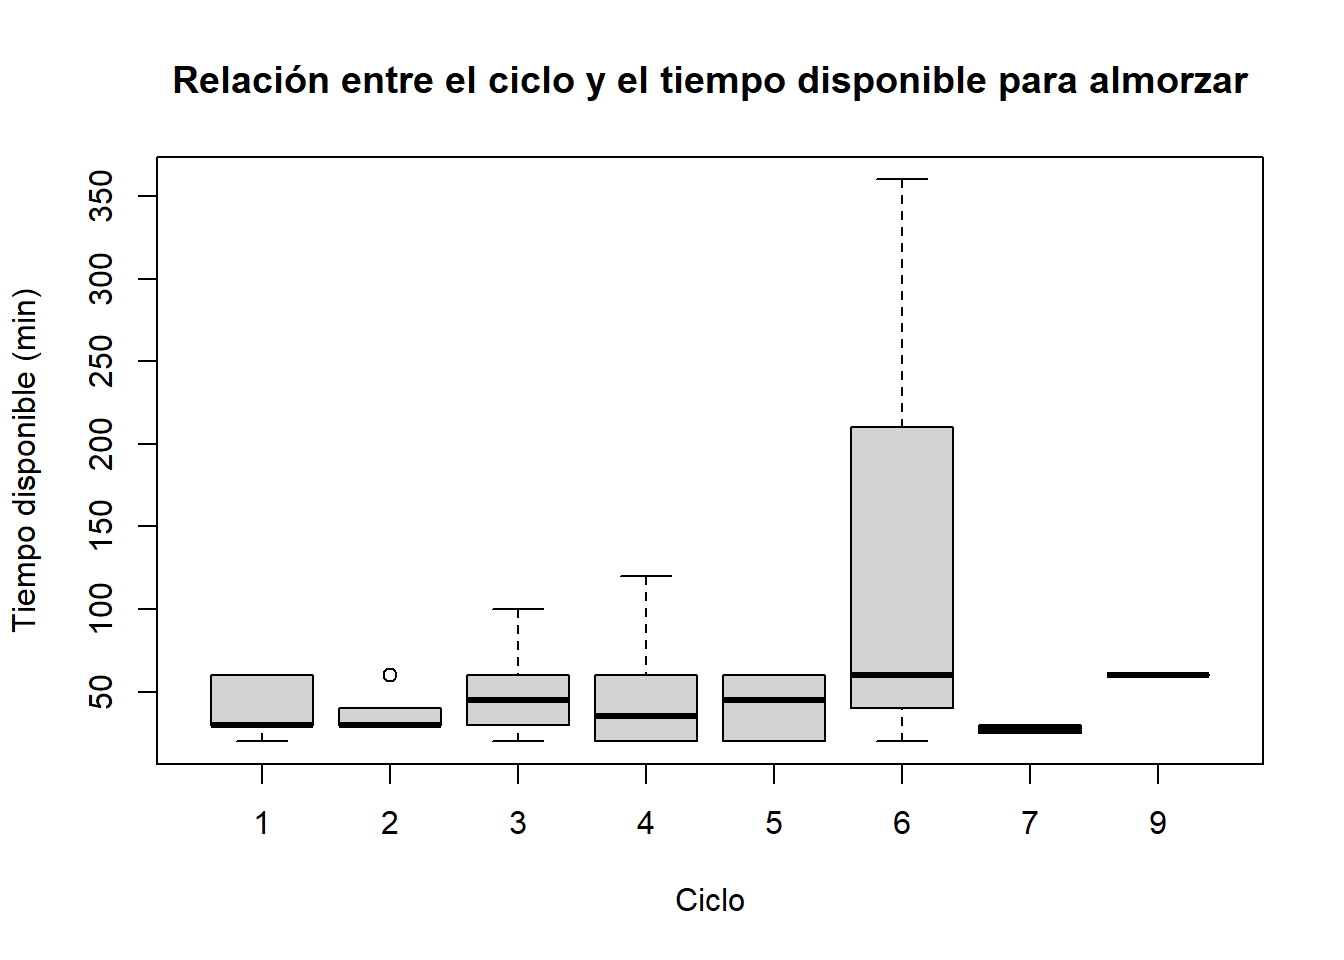
\includegraphics{S7_Infomre_E2_files/figure-latex/unnamed-chunk-27-1.pdf}

mas pisson, ver rubrica

\#\#MODELO POISSON

\begin{Shaded}
\begin{Highlighting}[]
\NormalTok{DFN}\SpecialCharTok{$}\NormalTok{Tiempo\_sin\_celular[DFN}\SpecialCharTok{$}\NormalTok{Tiempo\_sin\_celular }\SpecialCharTok{\textgreater{}}\DecValTok{700}\NormalTok{]}\OtherTok{\textless{}{-}} \ConstantTok{NA}
\FunctionTok{summary}\NormalTok{(DFN}\SpecialCharTok{$}\NormalTok{Tiempo\_sin\_celular)}
\end{Highlighting}
\end{Shaded}

\begin{verbatim}
##    Min. 1st Qu.  Median    Mean 3rd Qu.    Max.    NA's 
##    30.0   150.0   194.0   206.5   255.0   600.0       3
\end{verbatim}

Se observa que el tiempo mínimo para ver el celular luego de ponerlo a
cargar es de 30 mínimo por hora y en promedio lo vuelve a ver luego de 3
horas

En la Sala de Urgencias de un hospital se sabe que los pacientes llegan
según una Distribución de Poisson. Si se espera que lleguen 3 pacientes
cada hora. Calcule la probabilidad de que lleguen menos de 30 pacientes
durante las próximas 24 horas.

En los encuestados se sabe que usan su celular luego de cargarlo segun
una distribución de Poisson. Si se espera que lleguen a revizar su
celular 2 veces cada hora.Calcular la probabilidad de que menos de 100
encuestados llegue a ver su celular en las próximas 24 horas

En los encuestados se sabe que

\begin{Shaded}
\begin{Highlighting}[]
\NormalTok{l}\OtherTok{=}\DecValTok{2}\SpecialCharTok{*}\DecValTok{24}
\NormalTok{k}\OtherTok{=}\DecValTok{100{-}1}
\FunctionTok{plot}\NormalTok{(}\FunctionTok{dpois}\NormalTok{(}\DecValTok{0}\SpecialCharTok{:}\NormalTok{k,l),}\AttributeTok{col =} \StringTok{"orange"}\NormalTok{,}\AttributeTok{xlab=}\StringTok{"Cantidad de personas que no dejan de usar el celular por mas de 30 min en 1 hora"}\NormalTok{,}\AttributeTok{ylab=}\StringTok{"Probalidad DE POISSON"}\NormalTok{,}\AttributeTok{main =} \StringTok{"MODELO DE POISSON TIEMPO SIN USAR EL CULULAR"}\NormalTok{)}
\end{Highlighting}
\end{Shaded}

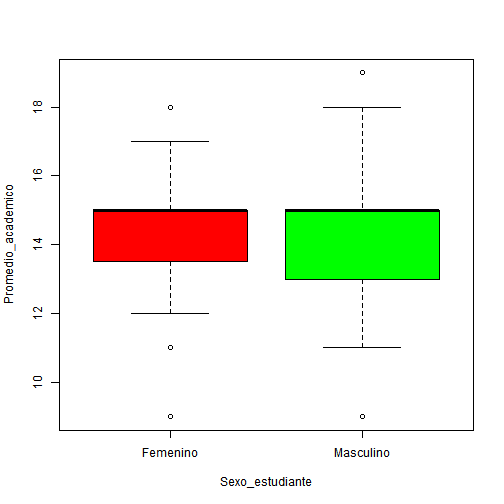
\includegraphics{S7_Infomre_E2_files/figure-latex/unnamed-chunk-29-1.pdf}

\end{document}
